\chapter{Relacions Trigonomètriques}\index{trigonometria}

\section{Funcions trigonomètriques}\index{funcions!trigonomètriques}

En la taula \vref{taula:func-trig-signes} es pot veure el signe de
les funcions trigonomètriques, segons en quin dels quatre quadrants
es trobi l'angle $\alpha$. \textbf{I}: $\alpha\in[0,\frac{\piup}{2}]$, \textbf{II}:
$\alpha\in[\frac{\piup}{2},\piup]$, \textbf{III}:
$\alpha\in[\piup,\frac{3\piup}{2}]$, \textbf{IV}:
$\alpha\in[\frac{3\piup}{2},2\piup]$.
\index{sin}\index{cos}\index{tan}\index{csc}\index{sec}\index{cot}

\begin{center}
   \captionof{table}{Signes de les funcions trigonomètriques en els quatre quadrants}
   \label{taula:func-trig-signes}
   \begin{tabular}{cccc|cccc}
   {\color{Green}$\sin\alpha \geq 0$} & {\color{Red}$\cos\alpha \leq 0$} & {\color{Red}$\tan\alpha \leq 0$} & & &
   {\color{Green}$\sin\alpha \geq 0$} & {\color{Green}$\cos\alpha \geq 0$} & {\color{Green}$\tan\alpha \geq 0$} \\
   {\color{Green}$\csc\alpha \geq 0$} & {\color{Red}$\sec\alpha \leq 0$} & {\color{Red}$\cot\alpha \leq 0$} & \textbf{II}&
   \textbf{I} & {\color{Green}$\csc\alpha \geq 0$} & {\color{Green}$\sec\alpha \geq 0$} & {\color{Green}$\cot\alpha \geq 0$} \\
   \hline
   {\color{Red}$\sin\alpha \leq 0$} & {\color{Red}$\cos\alpha \leq 0$} & {\color{Green}$\tan\alpha \geq 0$}
   &\textbf{III} &
   \textbf{IV} & {\color{Red}$\sin\alpha \leq 0$} & {\color{Green}$\cos\alpha \geq 0$} & {\color{Red}$\tan\alpha \leq 0$} \\
   {\color{Red}$\csc\alpha \leq 0$} & {\color{Red}$\sec\alpha \leq 0$} & {\color{Green}$\cot\alpha \geq 0$}  & & &
   {\color{Red}$\csc\alpha \leq 0$} & {\color{Green}$\sec\alpha \geq 0$} & {\color{Red}$\cot\alpha \leq 0$}
   \end{tabular}
\end{center}

En la taula \vref{taula:func-trig-angles} es pot veure el valor de
les funcions trigonomètriques per a diversos angles usuals.

\begin{center}
   \captionof{table}{Valors de les funcions trigonomètriques per a diversos angles} \label{taula:func-trig-angles}
   \begin{tabular}{cccccccc}
   \toprule[1pt]
    \multicolumn{2}{c}{$\alpha$} &
    \multirow{2}{15mm}{\hspace{2ex}\rule{0mm}{6mm}$\sin\alpha$} &
    \multirow{2}{15mm}{\hspace{2ex}\rule{0mm}{6mm}$\cos\alpha$}  &
    \multirow{2}{15mm}{\hspace{2ex}\rule{0mm}{6mm}$\tan\alpha$} &
    \multirow{2}{15mm}{\hspace{2ex}\rule{0mm}{6mm}$\csc\alpha$} &
    \multirow{2}{15mm}{\hspace{2ex}\rule{0mm}{6mm}$\sec\alpha$}  &
    \multirow{2}{15mm}{\hspace{2ex}\rule{0mm}{6mm}$\cot\alpha$}\\
    \cmidrule(rl){1-2}
    rad & \unit{\degree} & & & & & & \\
   \midrule
   0 & 0 & 0 & 1 & 0 & $\pm\infty$ & 1 & $\pm\infty$\\[1ex]
   $\dfrac{\piup}{6}$ & 30 & $\dfrac{1}{2}$ & $\dfrac{\sqrt{3}}{2}$ &
   $\dfrac{\sqrt{3}}{3}$ & 2 & $\dfrac{2\sqrt{3}}{3}$ & $\sqrt{3}$\\[1.5ex]
   $\dfrac{\piup}{4}$ & 45 & $\dfrac{\sqrt{2}}{2}$  &
   $\dfrac{\sqrt{2}}{2}$ & 1 & $\sqrt{2}$ & $\sqrt{2}$ & 1\\[1.5ex]
   $\dfrac{\piup}{3}$ & 60 &  $\dfrac{\sqrt{3}}{2}$ & $\dfrac{1}{2}$ &
   $\sqrt{3}$ & $\dfrac{2\sqrt{3}}{3}$ & 2 & $\dfrac{\sqrt{3}}{3}$\\[2ex]
   $\dfrac{\piup}{2}$ & 90 & 1 & 0 & $\pm\infty$ & 1 & $\pm\infty$ & 0\\[1.5ex]
   $\piup$ & 180 & 0 & $-1$ & 0 & $\pm\infty$ & $-1$ & $\pm\infty$\\[1ex]
   $\dfrac{3\piup}{2}$ & 270 & $-1$ & 0 & $\pm\infty$ & $-1$ & $\pm\infty$ & 0\\
   \bottomrule[1pt]
   \end{tabular}
\end{center}

 Es presenten a continuació  les funcions trigonomètriques d'angles en qualsevol
quadrant, en funció d'un angle en el primer quadrant,
$\alpha\in[0,\frac{\piup}{2}]$.
\begin{subequations}
\begin{align}
    \sin(-\alpha) &= -\sin\alpha  & \csc(-\alpha) &= -\csc\alpha \\[1.5ex]
    \cos(-\alpha) &= +\cos\alpha  & \sec(-\alpha) &= +\sec\alpha \\[1.5ex]
    \tan(-\alpha) &= -\tan\alpha  & \cot(-\alpha) &= -\cot\alpha
\end{align}
\end{subequations}
\vspace{-5mm}
\begin{subequations}
\begin{align}
    \sin\left(\frac{\piup}{2}\pm\alpha\right) &= +\cos\alpha    & \csc\left(\frac{\piup}{2}\pm\alpha\right) &= +\sec\alpha \\
    \cos\left(\frac{\piup}{2}\pm\alpha\right) &= \mp\sin\alpha  & \sec\left(\frac{\piup}{2}\pm\alpha\right) &= \mp\csc\alpha \\
    \tan\left(\frac{\piup}{2}\pm\alpha\right) &= \mp\cot\alpha  & \cot\left(\frac{\piup}{2}\pm\alpha\right) &= \mp\tan\alpha
\end{align}
\end{subequations}
\vspace{-5mm}
\begin{subequations}
\begin{align}
    \sin(\piup\pm\alpha) &= \mp\sin\alpha  & \csc(\piup\pm\alpha) &= \mp\csc\alpha \\[1.5ex]
    \cos(\piup\pm\alpha) &= -\cos\alpha    & \sec(\piup\pm\alpha) &= -\sec\alpha \\[1.5ex]
    \tan(\piup\pm\alpha) &= \pm\tan\alpha  & \cot(\piup\pm\alpha) &= \pm\cot\alpha
\end{align}
\end{subequations}
\vspace{-5mm}
\begin{subequations}
\begin{align}
    \sin\left(\frac{3\piup}{2}\pm\alpha\right) &= -\cos\alpha    & \csc\left(\frac{3\piup}{2}\pm\alpha\right) &= -\sec\alpha \\
    \cos\left(\frac{3\piup}{2}\pm\alpha\right) &= \pm\sin\alpha  & \sec\left(\frac{3\piup}{2}\pm\alpha\right) &= \pm\csc\alpha \\
    \tan\left(\frac{3\piup}{2}\pm\alpha\right) &= \mp\cot\alpha  & \cot\left(\frac{3\piup}{2}\pm\alpha\right) &= \mp\tan\alpha
\end{align}
\end{subequations}
\vspace{-5mm}
\begin{subequations}
\begin{align}
    \sin(2\piup\pm\alpha) &= \pm\sin\alpha  & \csc(2\piup\pm\alpha) &= \pm\csc\alpha \\
    \cos(2\piup\pm\alpha) &= +\cos\alpha    & \sec(2\piup\pm\alpha) &= +\sec\alpha \\
    \tan(2\piup\pm\alpha) &= \pm\tan\alpha  & \cot(2\piup\pm\alpha) &= \pm\cot\alpha
\end{align}
\end{subequations}




Es dona a continuació cadascuna de les funcions trigonomètriques en
funció de totes les altres. El signe «$\pm$» que apareix en les
equacions, ve determinat pel quadrant on es troba l'angle $\alpha$
(vegeu la taula \vref{taula:func-trig-signes}).
\begin{subequations}
\begin{align}
\sin\alpha &= \pm\sqrt{1-\cos^2\alpha} =
\frac{\tan\alpha}{\pm\sqrt{1+\tan^2\alpha}} =
\frac{1}{\pm\sqrt{1+\cot^2\alpha}} =
\frac{\pm\sqrt{\sec^2\alpha-1}}{\sec\alpha} = \frac{1}{\csc\alpha}\\[1.6ex]
\cos\alpha &= \pm\sqrt{1-\sin^2\alpha} =
\frac{1}{\pm\sqrt{1+\tan^2\alpha}} =
\frac{\cot\alpha}{\pm\sqrt{1+\cot^2\alpha}} = \frac{1}{\sec\alpha} =
\frac{\pm\sqrt{\csc^2\alpha-1}}{\csc\alpha}\\[1.6ex]
\tan\alpha &= \frac{\sin\alpha}{\pm\sqrt{1-\sin^2\alpha}} =
\frac{\pm\sqrt{1-\cos^2\alpha}}{\cos\alpha} = \frac{1}{\cot\alpha} =
\pm\sqrt{\sec^2\alpha-1} =
 \frac{1}{\pm\sqrt{\csc^2\alpha-1}}\displaybreak\\[1.6ex]
\csc\alpha &= \frac{1}{\sin\alpha} =
\frac{1}{\pm\sqrt{1-\cos^2\alpha}} =
\frac{\pm\sqrt{1+\tan^2\alpha}}{\tan\alpha} =
\pm\sqrt{1+\cot^2\alpha} =
\frac{\sec\alpha}{\pm\sqrt{\sec^2\alpha-1}}\\[1.6ex]
\sec\alpha &= \frac{1}{\pm\sqrt{1-\sin^2\alpha}} =
\frac{1}{\cos\alpha} = \pm\sqrt{1+\tan^2\alpha} =
\frac{\pm\sqrt{1+\cot^2\alpha}}{\cot\alpha} =
\frac{\csc\alpha}{\pm\sqrt{\csc^2\alpha-1}}\\[1.6ex]
\cot\alpha &= \frac{\pm\sqrt{1-\sin^2\alpha}}{\sin\alpha} =
\frac{\cos\alpha}{\pm\sqrt{1-\cos^2\alpha}} = \frac{1}{\tan\alpha} =
\frac{1}{\pm\sqrt{\sec^2\alpha-1}} = \pm\sqrt{\csc^2\alpha-1}
\end{align}
\end{subequations}

Identitats fonamentals de les funcions trigonomètriques:
\begin{gather}
    \sin^2\alpha + \cos^2\alpha = 1 \\
    1 + \tan^2\alpha = \sec^2\alpha\\
    1 + \cot^2\alpha = \csc^2\alpha\\
    \cos\alpha + j \sin\alpha = e^{j\alpha}
\end{gather}

Funcions trigonomètriques de l'angle doble, i generalització per a
$n\in\mathsfb{Z}$:
\begin{subequations}
\begin{align}
    \sin 2\alpha &= 2 \sin\alpha \cos\alpha & \sin n \alpha &=
    2\sin((n-1)\alpha)\cos \alpha -\sin((n-2)\alpha)\\[1ex]
    \cos 2\alpha &= 2\cos^2\alpha -1 & \cos n\alpha &=
    2\cos((n-1)\alpha)\cos \alpha -\cos((n-2)\alpha)\\[1ex]
    \tan 2\alpha &=\frac{2\tan\alpha}{1-\tan^2\alpha} & \tan n
    \alpha &= \frac{\tan((n-1)\alpha)+\tan\alpha}{1-\tan((n-1)\alpha)\tan\alpha}
\end{align}
\end{subequations}


Funcions trigonomètriques de l'angle meitat. El signe «$\pm$» que
apareix en les equacions, ve determinat pel quadrant on es troba
l'angle $\frac{\alpha}{2}$ (vegeu la taula
\vref{taula:func-trig-signes}):
\begin{subequations}
\begin{align}
    \sin \frac{\alpha}{2} &= \pm \sqrt{\frac{1-\cos\alpha}{2}}\\[1ex]
    \cos \frac{\alpha}{2} &= \pm \sqrt{\frac{1+\cos\alpha}{2}}\\[1ex]
    \tan \frac{\alpha}{2} &= \pm \sqrt{\frac{1-\cos\alpha}{1+\cos\alpha}}
\end{align}
\end{subequations}


Funcions trigonomètriques de la suma i diferència d'angles:
\begin{subequations}
\begin{align}
    \sin(\alpha+\beta) &= \sin\alpha \cos\beta + \sin\beta\cos\alpha &
    \sin(\alpha-\beta) &= \sin\alpha \cos\beta - \sin\beta\cos\alpha\\[1ex]
    \cos(\alpha+\beta) &= \cos\alpha \cos\beta - \sin\beta\sin\alpha &
    \cos(\alpha-\beta) &= \cos\alpha \cos\beta + \sin\beta\sin\alpha\label{eq:cos-a-b}\\[1ex]
    \tan(\alpha+\beta) &=\frac{\tan\alpha+\tan\beta}{1-\tan\alpha\tan\beta} &
    \tan(\alpha-\beta)
    &=\frac{\tan\alpha-\tan\beta}{1+\tan\alpha\tan\beta}
\end{align}
\end{subequations}

Suma i diferència de funcions trigonomètriques:
\begin{subequations}
\begin{align}
    \sin\alpha+\sin\beta &= 2 \sin\left(\frac{\alpha+\beta}{2}\right)
    \cos\left(\frac{\alpha-\beta}{2}\right)\\[1ex]
    \sin\alpha-\sin\beta &= 2 \cos\left(\frac{\alpha+\beta}{2}\right)
    \sin\left(\frac{\alpha-\beta}{2}\right)\\[1ex]
    \cos\alpha+\cos\beta &= 2 \cos\left(\frac{\alpha+\beta}{2}\right)
    \cos\left(\frac{\alpha-\beta}{2}\right)\\[1ex]
    \cos\alpha-\cos\beta &= -2 \sin\left(\frac{\alpha+\beta}{2}\right)
    \sin\left(\frac{\alpha-\beta}{2}\right)
\end{align}
\end{subequations}

Producte de funcions trigonomètriques:
\begin{subequations}
\begin{align}
    \sin\alpha \cos\beta &=
    \frac{\sin(\alpha-\beta)+\sin(\alpha+\beta)}{2}\\[1ex]
    \cos\alpha \cos\beta &=
    \frac{\cos(\alpha-\beta)+\cos(\alpha+\beta)}{2}\label{eq:cos-cos}\\[1ex]
    \sin\alpha \sin\beta &=
    \frac{\cos(\alpha-\beta)-\cos(\alpha+\beta)}{2}
\end{align}
\end{subequations}

Producte de funcions trigonomètriques de la suma i diferència
d'angles:
\begin{subequations}
\begin{align}
    \sin(\alpha+\beta) \sin(\alpha-\beta) &= \sin^2\alpha-\sin^2\beta =
    \cos^2\beta - \cos^2\alpha\\[1ex]
    \cos(\alpha+\beta) \cos(\alpha-\beta) &= \cos^2\alpha-\sin^2\beta =
    \cos^2\beta - \sin^2\alpha
\end{align}
\end{subequations}

Potències de funcions trigonomètriques:
\begin{subequations}
\begin{align}
    \sin^2\alpha &= \frac{1-\cos 2\alpha}{2} &  \cos^2\alpha &= \frac{1+\cos 2\alpha}{2}\\[1ex]
    \sin^3\alpha &= \frac{3\sin\alpha-\sin 3\alpha}{4} &  \cos^3\alpha &= \frac{3\cos\alpha+\cos 3\alpha}{4}\\[1ex]
    \sin^4\alpha &= \frac{3-4\cos 2\alpha+\cos 4\alpha}{8} &  \cos^4\alpha &= \frac{3+4\cos 2\alpha+\cos 4\alpha}{8}
\end{align}
\end{subequations}

Conversió de la suma d'una funció cosinus i una funció sinus, en una única
funció cosinus o sinus ($A,B\in\mathsfb{R}$):\footnote{Cal tenir en compte que la funció \texttt{arctan} disponible en moltes calculadores i llenguatges de programació, torna de forma estandarditzada valors compresos entre $-\frac{\piup}{2}$ i $\frac{\piup}{2}$. En aquest cas cal sumar el valor $\piup$, quan $A$ és negatiu, a l'angle obtingut amb la funció \textsf{arctan} per tal d'obtenir l'angle en el quadrant correcte.}
\begin{subequations}
\begin{align}
    A \cos \alpha + B \sin \alpha &= \sqrt{A^2+B^2}\, \cos \left(\alpha - \arctan\dfrac{B}{A}\right)\label{eq:AcosBsin}\\[1ex]
    A \cos \alpha + B \sin \alpha &= \sqrt{A^2+B^2}\, \sin \left(\alpha - \arctan\dfrac{B}{A}+\dfrac{\piup}{2}\right)\label{eq:AcosBsinS}
\end{align}
\end{subequations}

\break

\section{Lleis trigonomètriques dels triangles}\label{sec:lleis-trig-triang}

A continuació es presenten diverses lleis trigonomètriques relacionades amb els triangles. Aquestes lleis relacionen les longituds dels tres costats $a$, $b$ i $c$ d'un triangle qualsevol, com el de
la figura \vref{pic:llei-s-c-t}, amb els seus tres angles interiors
$\alpha$, $\beta$ i $\gamma$, i amb els radis $r$ i $R$ de les circumferències inscrita i circumscrita al triangle. $A$, $B$ i $C$ són els vèrtexs del triangle, $I$ és el centre de la circumferència inscrita, $O$   és el centre de la circumferència circumscrita, i $G$ és el baricentre del triangle. Finalment, $\mathscr{A}$ és l'àrea del triangle.

\begin{center}
    \input{Imatges/Ape-Trigonometria-Triangle.pdf_tex}
    \captionof{figure}{Lleis trigonomètriques dels triangles} \label{pic:llei-s-c-t}
\end{center}

Es defineix, en primer lloc, la quantitat $s$ com la semisuma dels tres costats del triangle:
\begin{equation}
	s \equiv \frac{a+b+c}{2}
\end{equation}

La distància entre els centres $I$ i $O$ és definida per l'expressió:
\begin{equation}
	\overline{IO} = R(R-2r)
\end{equation}

De l'expressió anterior es dedueix:
\begin{equation}
	R  \geq 2r
\end{equation}

Es donen a continuació algunes expressions\footnote{L'equació \eqref{eq:Hero1} es coneix amb el nom de \emph{fórmula d'Heró}, pel matemàtic grecoromà Heró d'Alexandria: \href{https://en.wikipedia.org/wiki/Hero_of_Alexandria}{https:/\!\!/en.wikipedia.org/wiki/Hero\_of\_Alexandria}. L'equació \eqref{eq:Hero2} és una variant  de la \eqref{eq:Hero1}, que és més precisa per a valors molt petits d'un costat respecte dels altres dos; cal mantenir tots els parèntesis a l'hora de fer els càlculs.} que relacionen els dos radis $r$ i $R$, i els tres costats $a$, $b$ i $c$,  amb l'àrea $\mathscr{A}$.
\index{formula@fórmula!d'Heró}\index{area@àrea}\index{A@$\mathscr{A}$}
\begin{align}
	\mathscr{A} &= \sqrt{s (s-a) (s-b) (s-c)} \label{eq:Hero1} \\
	\mathscr{A} &=\frac{1}{4} \sqrt{(a+(b+c)) (c-(a-b) (c+(a-b)) (a+(b-c))}, \quad a \geq b\geq c \label{eq:Hero2}\\
	\mathscr{A} &= r s \\ 
	\mathscr{A} &= \frac{a b c}{4R} 
\end{align}

La llei dels sinus ens dona les relacions següents:\index{llei!dels
sinus}
\begin{equation}
    \frac{a}{\sin\alpha} = \frac{b}{\sin\beta} =
    \frac{c}{\sin\gamma} = 2 R = \frac{a b c}{2\,\mathscr{A}}
\end{equation}

La llei dels cosinus ens dona les relacions següents:\index{llei!dels cosinus}
\begin{subequations}
\begin{align}
    a^2 &= b^2 + c^2 - 2 b c \cos\alpha \\[1ex]
    b^2 &= a^2 + c^2 - 2 a c \cos\beta \\[1ex]
    c^2 &= a^2 + b^2 - 2 a b \cos\gamma
\end{align}
\end{subequations}

La llei de les tangents ens dona les relacions següents:\index{llei!de les tangents}
\begin{subequations}
\begin{align}
    \frac{a-b}{a+b} &= \frac{\tan\frac{\alpha-\beta}{2}}{\tan\frac{\alpha+\beta}{2}} \\[1ex]
    \frac{a-c}{a+c} &= \frac{\tan\frac{\alpha-\gamma}{2}}{\tan\frac{\alpha+\gamma}{2}} \\[1ex]
    \frac{b-c}{b+c} &= \frac{\tan\frac{\beta-\gamma}{2}}{\tan\frac{\beta+\gamma}{2}}
\end{align}
\end{subequations}

La llei de les cotangents ens dona les relacions següents:\index{llei!de les cotangents}
\begin{equation}
    \frac{b+c-a}{\cot\frac{\alpha}{2}} = \frac{a+c-b}{\cot\frac{\beta}{2}} =
    \frac{a+b-c}{\cot\frac{\gamma}{2}} = 2 r = \frac{2\,\mathscr{A} }{s}
\end{equation}

La fórmula de Mollweide,\footnote{Karl Mollweide, matemàtic alemany: \href{https://en.wikipedia.org/wiki/Karl_Mollweide}{https:/\!\!/en.wikipedia.org/wiki/Karl\_Mollweide}.} la qual lliga els tres costats amb els tres angles interiors d'un triangle, ens dona les relacions següents:\index{formula@fórmula!de Mollweide}
\begin{subequations}
\begin{align}
    \frac{a+b}{c} &= \frac{\cos\frac{\alpha-\beta}{2}}{\sin\frac{\gamma}{2}} \\[1ex]
    \frac{a-b}{c} &= \frac{\sin\frac{\alpha-\beta}{2}}{\cos\frac{\gamma}{2}}
\end{align}
\end{subequations}

Tal com s'ha dit en la secció \vref{sec:comp-sim-neutre}, el baricentre del triangle format per tres tensions fase-fase és el punt neutre de l'únic sistema de tres tensions fase-neutre que no té components homopolars. El baricentre és de fet, el centre de masses del triangle ---considerant-lo com una figura geomètrica massissa de densitat uniforme.  Les coordenades cartesianes del baricentre $(G_x,G_y)$ es calculen a partir de les coordenades cartesianes dels tres vèrtexs $(A_x,A_y)$, $(B_x,B_y)$ i $(C_x,C_y)$ segons:\index{baricentre}
\begin{subequations}
\begin{align}
    G_x &= \frac{A_x + B_x + C_x}{3} \label{eq:bari_x}\\[1ex]
    G_y &= \frac{A_y + B_y + C_y}{3} \label{eq:bari_y}
\end{align}
\end{subequations}


\section{Funcions hiperbòliques}\index{funcions!hiperbòliques}

Definició de les funcions hiperbòliques ($z\in\mathsfb{C}$):
\begin{subequations}
\begin{align}
    \sinh z&\equiv \frac{e^z - e^{-z}}{2} \\[1ex]
    \cosh z&\equiv \frac{e^z + e^{-z}}{2} \\[1ex]
    \tanh z&\equiv \frac{\sinh z}{\cosh z} = \frac{e^{2z}-1}{e^{2z}+1} \\[1ex]
    \csch z &\equiv\frac{1}{\sinh z} =
    \frac{2}{e^z - e^{-z}} \\[1ex]
    \sech z &\equiv\frac{1}{\cosh z} =
    \frac{2}{e^z + e^{-z}} \\[1ex]
    \coth z &\equiv\frac{1}{\tanh z} = \frac{e^{2z}+1}{e^{2z}-1}
\end{align}
\end{subequations}
\index{sinh}\index{cosh}\index{tanh}\index{csch}\index{sech}\index{coth}

Relacions entre les funcions trigonomètriques i les  hiperbòliques ($z\in\mathsfb{C}$):
\begin{subequations}
	\begin{align}
		\sin (j z) &= j \sinh z \\[1ex] 
		\cos (j z) &= \cosh z \\[1ex] 
		\tan (j z) &= j \tanh z \\[1ex] 
		\csc (j z) &= -j \csch z \\[1ex]
		\sec (j z) &=  \sech z \\[1ex]
		\cot (j z) &= -j \coth z
	\end{align}
\end{subequations}

Identitats fonamentals de les funcions hiperbòliques
($z\in\mathsfb{C}$):
\begin{align}
    &\cosh^2 z - \sinh^2 z = 1 \\
    &\sech^2 z + \tanh^2 z = 1 \\
    &\csch^2 z - \coth^2 z = -1 \\
    &\cosh z + \sinh z = e^z
\end{align}

Les funcions hiperbòliques presenten les següents simetries
($z\in\mathsfb{C}$):
\begin{subequations}
\begin{align}
    \sinh (-z) &= -\sinh z \\
    \cosh (-z) &= \cosh z\\
    \tanh (-z) &= -\tanh z
\end{align}
\end{subequations}

Funcions hiperbòliques de la suma i diferència d'arguments ($z_1,
z_2\in\mathsfb{C}$):
\begin{subequations}
\begin{align}
    \sinh(z_1+z_2) &= \sinh z_1 \cosh z_2 + \sinh z_2\cosh z_1\\[1ex]
    \sinh(z_1-z_2) &= \sinh z_1 \cosh z_2 - \sinh z_2\cosh z_1\\[1ex]
    \cosh(z_1+z_2) &= \cosh z_1 \cosh z_2 + \sinh z_2\sinh z_1\\[1ex]
    \cosh(z_1-z_2) &= \cosh z_1 \cosh z_2 - \sinh z_2\sinh z_1\\[1ex]
    \tanh(z_1+z_2) &=\frac{\tanh z_1+\tanh z_2}{1+\tanh z_1\tanh z_2}\\[1ex]
    \tanh(z_1-z_2) &=\frac{\tanh z_1-\tanh z_2}{1-\tanh z_1\tanh z_2}
\end{align}
\end{subequations}

Suma i diferència de funcions hiperbòliques ($z_1,
z_2\in\mathsfb{C}$):
\begin{subequations}
\begin{align}
    \sinh z_1+\sinh z_2 &= 2 \sinh\left(\frac{z_1+z_2}{2}\right)
    \cosh\left(\frac{z_1-z_2}{2}\right)\\[1ex]
    \sinh z_1-\sinh z_2 &= 2 \cosh\left(\frac{z_1+z_2}{2}\right)
    \sinh\left(\frac{z_1-z_2}{2}\right)\\[1ex]
    \cosh z_1+\cosh z_2 &= 2 \cosh\left(\frac{z_1+z_2}{2}\right)
    \cosh\left(\frac{z_1-z_2}{2}\right)\\[1ex]
    \cosh z_1-\cosh z_2 &= 2 \sinh\left(\frac{z_1+z_2}{2}\right)
    \sinh\left(\frac{z_1-z_2}{2}\right)
\end{align}
\end{subequations}

Producte de funcions hiperbòliques ($z_1, z_2\in\mathsfb{C}$):
\begin{subequations}
\begin{align}
    \sinh z_1 \cosh z_2 &=
    \frac{\sinh(z_1+z_2)+\sinh(z_1-z_2)}{2}\\[1ex]
    \cosh z_1 \cosh z_2 &=
    \frac{\cosh(z_1+z_2)+\cosh(z_1-z_2)}{2}\\[1ex]
    \sinh z_1 \sinh z_2 &=
    \frac{\cosh(z_1+z_2)-\cosh(z_1-z_2)}{2}
\end{align}
\end{subequations}


\section{Gràfiques}\label{sec:trig-grafics}

Es representen a continuació les gràfiques de les funcions trigonomètriques i hiperbòliques, per a valors reals.

\begin{center}
	% GNUPLOT: LaTeX picture with Postscript
\begingroup
  \makeatletter
  \providecommand\color[2][]{%
    \GenericError{(gnuplot) \space\space\space\@spaces}{%
      Package color not loaded in conjunction with
      terminal option `colourtext'%
    }{See the gnuplot documentation for explanation.%
    }{Either use 'blacktext' in gnuplot or load the package
      color.sty in LaTeX.}%
    \renewcommand\color[2][]{}%
  }%
  \providecommand\includegraphics[2][]{%
    \GenericError{(gnuplot) \space\space\space\@spaces}{%
      Package graphicx or graphics not loaded%
    }{See the gnuplot documentation for explanation.%
    }{The gnuplot epslatex terminal needs graphicx.sty or graphics.sty.}%
    \renewcommand\includegraphics[2][]{}%
  }%
  \providecommand\rotatebox[2]{#2}%
  \@ifundefined{ifGPcolor}{%
    \newif\ifGPcolor
    \GPcolortrue
  }{}%
  \@ifundefined{ifGPblacktext}{%
    \newif\ifGPblacktext
    \GPblacktexttrue
  }{}%
  % define a \g@addto@macro without @ in the name:
  \let\gplgaddtomacro\g@addto@macro
  % define empty templates for all commands taking text:
  \gdef\gplbacktext{}%
  \gdef\gplfronttext{}%
  \makeatother
  \ifGPblacktext
    % no textcolor at all
    \def\colorrgb#1{}%
    \def\colorgray#1{}%
  \else
    % gray or color?
    \ifGPcolor
      \def\colorrgb#1{\color[rgb]{#1}}%
      \def\colorgray#1{\color[gray]{#1}}%
      \expandafter\def\csname LTw\endcsname{\color{white}}%
      \expandafter\def\csname LTb\endcsname{\color{black}}%
      \expandafter\def\csname LTa\endcsname{\color{black}}%
      \expandafter\def\csname LT0\endcsname{\color[rgb]{1,0,0}}%
      \expandafter\def\csname LT1\endcsname{\color[rgb]{0,1,0}}%
      \expandafter\def\csname LT2\endcsname{\color[rgb]{0,0,1}}%
      \expandafter\def\csname LT3\endcsname{\color[rgb]{1,0,1}}%
      \expandafter\def\csname LT4\endcsname{\color[rgb]{0,1,1}}%
      \expandafter\def\csname LT5\endcsname{\color[rgb]{1,1,0}}%
      \expandafter\def\csname LT6\endcsname{\color[rgb]{0,0,0}}%
      \expandafter\def\csname LT7\endcsname{\color[rgb]{1,0.3,0}}%
      \expandafter\def\csname LT8\endcsname{\color[rgb]{0.5,0.5,0.5}}%
    \else
      % gray
      \def\colorrgb#1{\color{black}}%
      \def\colorgray#1{\color[gray]{#1}}%
      \expandafter\def\csname LTw\endcsname{\color{white}}%
      \expandafter\def\csname LTb\endcsname{\color{black}}%
      \expandafter\def\csname LTa\endcsname{\color{black}}%
      \expandafter\def\csname LT0\endcsname{\color{black}}%
      \expandafter\def\csname LT1\endcsname{\color{black}}%
      \expandafter\def\csname LT2\endcsname{\color{black}}%
      \expandafter\def\csname LT3\endcsname{\color{black}}%
      \expandafter\def\csname LT4\endcsname{\color{black}}%
      \expandafter\def\csname LT5\endcsname{\color{black}}%
      \expandafter\def\csname LT6\endcsname{\color{black}}%
      \expandafter\def\csname LT7\endcsname{\color{black}}%
      \expandafter\def\csname LT8\endcsname{\color{black}}%
    \fi
  \fi
    \setlength{\unitlength}{0.0500bp}%
    \ifx\gptboxheight\undefined%
      \newlength{\gptboxheight}%
      \newlength{\gptboxwidth}%
      \newsavebox{\gptboxtext}%
    \fi%
    \setlength{\fboxrule}{0.5pt}%
    \setlength{\fboxsep}{1pt}%
    \definecolor{tbcol}{rgb}{1,1,1}%
\begin{picture}(8500.00,5380.00)%
    \gplgaddtomacro\gplbacktext{%
      \colorrgb{0.00,0.00,0.00}%%
      \put(837,764){\makebox(0,0)[r]{\strut{}-1,00}}%
      \colorrgb{0.00,0.00,0.00}%%
      \put(837,1312){\makebox(0,0)[r]{\strut{}-0,75}}%
      \colorrgb{0.00,0.00,0.00}%%
      \put(837,1860){\makebox(0,0)[r]{\strut{}-0,50}}%
      \colorrgb{0.00,0.00,0.00}%%
      \put(837,2408){\makebox(0,0)[r]{\strut{}-0,25}}%
      \colorrgb{0.00,0.00,0.00}%%
      \put(837,2956){\makebox(0,0)[r]{\strut{} 0,00}}%
      \colorrgb{0.00,0.00,0.00}%%
      \put(837,3503){\makebox(0,0)[r]{\strut{} 0,25}}%
      \colorrgb{0.00,0.00,0.00}%%
      \put(837,4051){\makebox(0,0)[r]{\strut{} 0,50}}%
      \colorrgb{0.00,0.00,0.00}%%
      \put(837,4599){\makebox(0,0)[r]{\strut{} 0,75}}%
      \colorrgb{0.00,0.00,0.00}%%
      \put(837,5147){\makebox(0,0)[r]{\strut{} 1,00}}%
      \colorrgb{0.00,0.00,0.00}%%
      \put(1018,467){\makebox(0,0){\strut{}-$2\pi$}}%
      \colorrgb{0.00,0.00,0.00}%%
      \put(1901,467){\makebox(0,0){\strut{}-$\frac{3\pi}{2}$}}%
      \colorrgb{0.00,0.00,0.00}%%
      \put(2784,467){\makebox(0,0){\strut{}-$\pi$}}%
      \colorrgb{0.00,0.00,0.00}%%
      \put(3668,467){\makebox(0,0){\strut{}-$\frac{\pi}{2}$}}%
      \colorrgb{0.00,0.00,0.00}%%
      \put(4551,467){\makebox(0,0){\strut{}$0$}}%
      \colorrgb{0.00,0.00,0.00}%%
      \put(5435,467){\makebox(0,0){\strut{}$\frac{\pi}{2}$}}%
      \colorrgb{0.00,0.00,0.00}%%
      \put(6318,467){\makebox(0,0){\strut{}$\pi$}}%
      \colorrgb{0.00,0.00,0.00}%%
      \put(7202,467){\makebox(0,0){\strut{}$\frac{3\pi}{2}$}}%
      \colorrgb{0.00,0.00,0.00}%%
      \put(8085,467){\makebox(0,0){\strut{}$2\pi$}}%
    }%
    \gplgaddtomacro\gplfronttext{%
      \csname LTb\endcsname%%
      \put(178,2956){\rotatebox{-270}{\makebox(0,0){\strut{}$\sin \alpha$}}}%
      \csname LTb\endcsname%%
      \put(8138,2956){\rotatebox{-270}{\makebox(0,0){\strut{}}}}%
      \csname LTb\endcsname%%
      \put(4551,148){\makebox(0,0){\strut{}$\alpha$}}%
      \csname LTb\endcsname%%
      \put(4551,5147){\makebox(0,0){\strut{}}}%
      \csname LTb\endcsname%%
      \put(4551,5147){\makebox(0,0){\strut{}}}%
    }%
    \gplbacktext
    \put(0,0){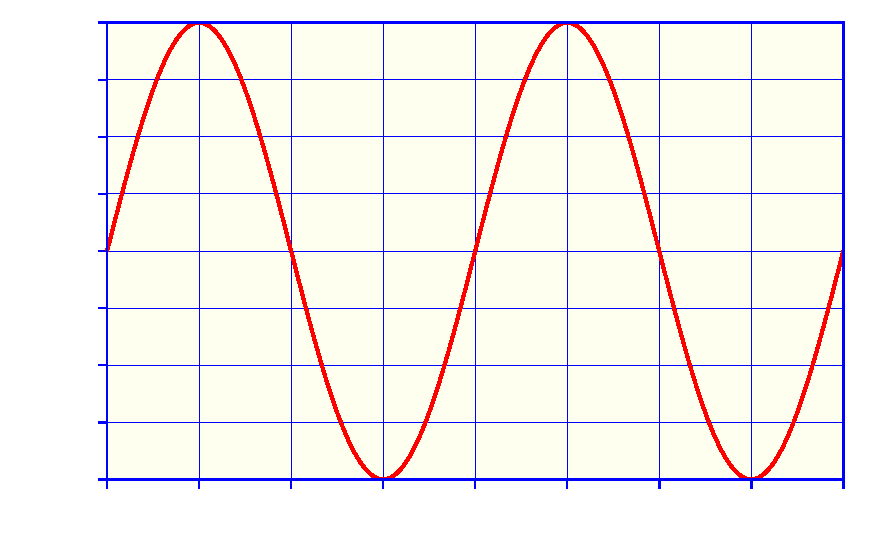
\includegraphics[width={425.00bp},height={269.00bp}]{Ape-Trigonometria-sin}}%
    \gplfronttext
  \end{picture}%
\endgroup

	\captionof{figure}{Funció sinus} 
\end{center}

\begin{center}
	% GNUPLOT: LaTeX picture with Postscript
\begingroup
  \makeatletter
  \providecommand\color[2][]{%
    \GenericError{(gnuplot) \space\space\space\@spaces}{%
      Package color not loaded in conjunction with
      terminal option `colourtext'%
    }{See the gnuplot documentation for explanation.%
    }{Either use 'blacktext' in gnuplot or load the package
      color.sty in LaTeX.}%
    \renewcommand\color[2][]{}%
  }%
  \providecommand\includegraphics[2][]{%
    \GenericError{(gnuplot) \space\space\space\@spaces}{%
      Package graphicx or graphics not loaded%
    }{See the gnuplot documentation for explanation.%
    }{The gnuplot epslatex terminal needs graphicx.sty or graphics.sty.}%
    \renewcommand\includegraphics[2][]{}%
  }%
  \providecommand\rotatebox[2]{#2}%
  \@ifundefined{ifGPcolor}{%
    \newif\ifGPcolor
    \GPcolortrue
  }{}%
  \@ifundefined{ifGPblacktext}{%
    \newif\ifGPblacktext
    \GPblacktexttrue
  }{}%
  % define a \g@addto@macro without @ in the name:
  \let\gplgaddtomacro\g@addto@macro
  % define empty templates for all commands taking text:
  \gdef\gplbacktext{}%
  \gdef\gplfronttext{}%
  \makeatother
  \ifGPblacktext
    % no textcolor at all
    \def\colorrgb#1{}%
    \def\colorgray#1{}%
  \else
    % gray or color?
    \ifGPcolor
      \def\colorrgb#1{\color[rgb]{#1}}%
      \def\colorgray#1{\color[gray]{#1}}%
      \expandafter\def\csname LTw\endcsname{\color{white}}%
      \expandafter\def\csname LTb\endcsname{\color{black}}%
      \expandafter\def\csname LTa\endcsname{\color{black}}%
      \expandafter\def\csname LT0\endcsname{\color[rgb]{1,0,0}}%
      \expandafter\def\csname LT1\endcsname{\color[rgb]{0,1,0}}%
      \expandafter\def\csname LT2\endcsname{\color[rgb]{0,0,1}}%
      \expandafter\def\csname LT3\endcsname{\color[rgb]{1,0,1}}%
      \expandafter\def\csname LT4\endcsname{\color[rgb]{0,1,1}}%
      \expandafter\def\csname LT5\endcsname{\color[rgb]{1,1,0}}%
      \expandafter\def\csname LT6\endcsname{\color[rgb]{0,0,0}}%
      \expandafter\def\csname LT7\endcsname{\color[rgb]{1,0.3,0}}%
      \expandafter\def\csname LT8\endcsname{\color[rgb]{0.5,0.5,0.5}}%
    \else
      % gray
      \def\colorrgb#1{\color{black}}%
      \def\colorgray#1{\color[gray]{#1}}%
      \expandafter\def\csname LTw\endcsname{\color{white}}%
      \expandafter\def\csname LTb\endcsname{\color{black}}%
      \expandafter\def\csname LTa\endcsname{\color{black}}%
      \expandafter\def\csname LT0\endcsname{\color{black}}%
      \expandafter\def\csname LT1\endcsname{\color{black}}%
      \expandafter\def\csname LT2\endcsname{\color{black}}%
      \expandafter\def\csname LT3\endcsname{\color{black}}%
      \expandafter\def\csname LT4\endcsname{\color{black}}%
      \expandafter\def\csname LT5\endcsname{\color{black}}%
      \expandafter\def\csname LT6\endcsname{\color{black}}%
      \expandafter\def\csname LT7\endcsname{\color{black}}%
      \expandafter\def\csname LT8\endcsname{\color{black}}%
    \fi
  \fi
    \setlength{\unitlength}{0.0500bp}%
    \ifx\gptboxheight\undefined%
      \newlength{\gptboxheight}%
      \newlength{\gptboxwidth}%
      \newsavebox{\gptboxtext}%
    \fi%
    \setlength{\fboxrule}{0.5pt}%
    \setlength{\fboxsep}{1pt}%
    \definecolor{tbcol}{rgb}{1,1,1}%
\begin{picture}(8500.00,5380.00)%
    \gplgaddtomacro\gplbacktext{%
      \colorrgb{0.00,0.00,0.00}%%
      \put(548,764){\makebox(0,0)[r]{\strut{}-5}}%
      \colorrgb{0.00,0.00,0.00}%%
      \put(548,1202){\makebox(0,0)[r]{\strut{}-4}}%
      \colorrgb{0.00,0.00,0.00}%%
      \put(548,1641){\makebox(0,0)[r]{\strut{}-3}}%
      \colorrgb{0.00,0.00,0.00}%%
      \put(548,2079){\makebox(0,0)[r]{\strut{}-2}}%
      \colorrgb{0.00,0.00,0.00}%%
      \put(548,2517){\makebox(0,0)[r]{\strut{}-1}}%
      \colorrgb{0.00,0.00,0.00}%%
      \put(548,2956){\makebox(0,0)[r]{\strut{} 0}}%
      \colorrgb{0.00,0.00,0.00}%%
      \put(548,3394){\makebox(0,0)[r]{\strut{} 1}}%
      \colorrgb{0.00,0.00,0.00}%%
      \put(548,3832){\makebox(0,0)[r]{\strut{} 2}}%
      \colorrgb{0.00,0.00,0.00}%%
      \put(548,4270){\makebox(0,0)[r]{\strut{} 3}}%
      \colorrgb{0.00,0.00,0.00}%%
      \put(548,4709){\makebox(0,0)[r]{\strut{} 4}}%
      \colorrgb{0.00,0.00,0.00}%%
      \put(548,5147){\makebox(0,0)[r]{\strut{} 5}}%
      \colorrgb{0.00,0.00,0.00}%%
      \put(729,467){\makebox(0,0){\strut{}-$2\pi$}}%
      \colorrgb{0.00,0.00,0.00}%%
      \put(1649,467){\makebox(0,0){\strut{}-$\frac{3\pi}{2}$}}%
      \colorrgb{0.00,0.00,0.00}%%
      \put(2568,467){\makebox(0,0){\strut{}-$\pi$}}%
      \colorrgb{0.00,0.00,0.00}%%
      \put(3488,467){\makebox(0,0){\strut{}-$\frac{\pi}{2}$}}%
      \colorrgb{0.00,0.00,0.00}%%
      \put(4407,467){\makebox(0,0){\strut{}$0$}}%
      \colorrgb{0.00,0.00,0.00}%%
      \put(5327,467){\makebox(0,0){\strut{}$\frac{\pi}{2}$}}%
      \colorrgb{0.00,0.00,0.00}%%
      \put(6246,467){\makebox(0,0){\strut{}$\pi$}}%
      \colorrgb{0.00,0.00,0.00}%%
      \put(7165,467){\makebox(0,0){\strut{}$\frac{3\pi}{2}$}}%
      \colorrgb{0.00,0.00,0.00}%%
      \put(8085,467){\makebox(0,0){\strut{}$2\pi$}}%
    }%
    \gplgaddtomacro\gplfronttext{%
      \csname LTb\endcsname%%
      \put(178,2956){\rotatebox{-270}{\makebox(0,0){\strut{}$\csc \alpha$}}}%
      \csname LTb\endcsname%%
      \put(8138,2956){\rotatebox{-270}{\makebox(0,0){\strut{}}}}%
      \csname LTb\endcsname%%
      \put(4407,148){\makebox(0,0){\strut{}$\alpha$}}%
      \csname LTb\endcsname%%
      \put(4407,5147){\makebox(0,0){\strut{}}}%
      \csname LTb\endcsname%%
      \put(4407,5147){\makebox(0,0){\strut{}}}%
    }%
    \gplbacktext
    \put(0,0){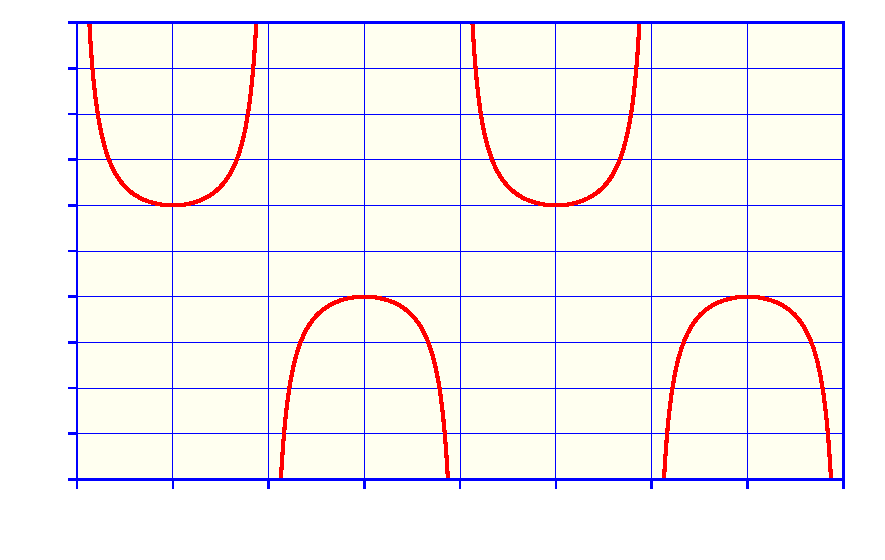
\includegraphics[width={425.00bp},height={269.00bp}]{Ape-Trigonometria-csc}}%
    \gplfronttext
  \end{picture}%
\endgroup

	\captionof{figure}{Funció cosecant} 
\end{center}

\vspace{5mm}
\begin{center}
	% GNUPLOT: LaTeX picture with Postscript
\begingroup
  \makeatletter
  \providecommand\color[2][]{%
    \GenericError{(gnuplot) \space\space\space\@spaces}{%
      Package color not loaded in conjunction with
      terminal option `colourtext'%
    }{See the gnuplot documentation for explanation.%
    }{Either use 'blacktext' in gnuplot or load the package
      color.sty in LaTeX.}%
    \renewcommand\color[2][]{}%
  }%
  \providecommand\includegraphics[2][]{%
    \GenericError{(gnuplot) \space\space\space\@spaces}{%
      Package graphicx or graphics not loaded%
    }{See the gnuplot documentation for explanation.%
    }{The gnuplot epslatex terminal needs graphicx.sty or graphics.sty.}%
    \renewcommand\includegraphics[2][]{}%
  }%
  \providecommand\rotatebox[2]{#2}%
  \@ifundefined{ifGPcolor}{%
    \newif\ifGPcolor
    \GPcolortrue
  }{}%
  \@ifundefined{ifGPblacktext}{%
    \newif\ifGPblacktext
    \GPblacktexttrue
  }{}%
  % define a \g@addto@macro without @ in the name:
  \let\gplgaddtomacro\g@addto@macro
  % define empty templates for all commands taking text:
  \gdef\gplbacktext{}%
  \gdef\gplfronttext{}%
  \makeatother
  \ifGPblacktext
    % no textcolor at all
    \def\colorrgb#1{}%
    \def\colorgray#1{}%
  \else
    % gray or color?
    \ifGPcolor
      \def\colorrgb#1{\color[rgb]{#1}}%
      \def\colorgray#1{\color[gray]{#1}}%
      \expandafter\def\csname LTw\endcsname{\color{white}}%
      \expandafter\def\csname LTb\endcsname{\color{black}}%
      \expandafter\def\csname LTa\endcsname{\color{black}}%
      \expandafter\def\csname LT0\endcsname{\color[rgb]{1,0,0}}%
      \expandafter\def\csname LT1\endcsname{\color[rgb]{0,1,0}}%
      \expandafter\def\csname LT2\endcsname{\color[rgb]{0,0,1}}%
      \expandafter\def\csname LT3\endcsname{\color[rgb]{1,0,1}}%
      \expandafter\def\csname LT4\endcsname{\color[rgb]{0,1,1}}%
      \expandafter\def\csname LT5\endcsname{\color[rgb]{1,1,0}}%
      \expandafter\def\csname LT6\endcsname{\color[rgb]{0,0,0}}%
      \expandafter\def\csname LT7\endcsname{\color[rgb]{1,0.3,0}}%
      \expandafter\def\csname LT8\endcsname{\color[rgb]{0.5,0.5,0.5}}%
    \else
      % gray
      \def\colorrgb#1{\color{black}}%
      \def\colorgray#1{\color[gray]{#1}}%
      \expandafter\def\csname LTw\endcsname{\color{white}}%
      \expandafter\def\csname LTb\endcsname{\color{black}}%
      \expandafter\def\csname LTa\endcsname{\color{black}}%
      \expandafter\def\csname LT0\endcsname{\color{black}}%
      \expandafter\def\csname LT1\endcsname{\color{black}}%
      \expandafter\def\csname LT2\endcsname{\color{black}}%
      \expandafter\def\csname LT3\endcsname{\color{black}}%
      \expandafter\def\csname LT4\endcsname{\color{black}}%
      \expandafter\def\csname LT5\endcsname{\color{black}}%
      \expandafter\def\csname LT6\endcsname{\color{black}}%
      \expandafter\def\csname LT7\endcsname{\color{black}}%
      \expandafter\def\csname LT8\endcsname{\color{black}}%
    \fi
  \fi
    \setlength{\unitlength}{0.0500bp}%
    \ifx\gptboxheight\undefined%
      \newlength{\gptboxheight}%
      \newlength{\gptboxwidth}%
      \newsavebox{\gptboxtext}%
    \fi%
    \setlength{\fboxrule}{0.5pt}%
    \setlength{\fboxsep}{1pt}%
    \definecolor{tbcol}{rgb}{1,1,1}%
\begin{picture}(8500.00,5380.00)%
    \gplgaddtomacro\gplbacktext{%
      \colorrgb{0.00,0.00,0.00}%%
      \put(837,764){\makebox(0,0)[r]{\strut{}-1,00}}%
      \colorrgb{0.00,0.00,0.00}%%
      \put(837,1312){\makebox(0,0)[r]{\strut{}-0,75}}%
      \colorrgb{0.00,0.00,0.00}%%
      \put(837,1860){\makebox(0,0)[r]{\strut{}-0,50}}%
      \colorrgb{0.00,0.00,0.00}%%
      \put(837,2408){\makebox(0,0)[r]{\strut{}-0,25}}%
      \colorrgb{0.00,0.00,0.00}%%
      \put(837,2956){\makebox(0,0)[r]{\strut{} 0,00}}%
      \colorrgb{0.00,0.00,0.00}%%
      \put(837,3503){\makebox(0,0)[r]{\strut{} 0,25}}%
      \colorrgb{0.00,0.00,0.00}%%
      \put(837,4051){\makebox(0,0)[r]{\strut{} 0,50}}%
      \colorrgb{0.00,0.00,0.00}%%
      \put(837,4599){\makebox(0,0)[r]{\strut{} 0,75}}%
      \colorrgb{0.00,0.00,0.00}%%
      \put(837,5147){\makebox(0,0)[r]{\strut{} 1,00}}%
      \colorrgb{0.00,0.00,0.00}%%
      \put(1018,467){\makebox(0,0){\strut{}-$2\pi$}}%
      \colorrgb{0.00,0.00,0.00}%%
      \put(1901,467){\makebox(0,0){\strut{}-$\frac{3\pi}{2}$}}%
      \colorrgb{0.00,0.00,0.00}%%
      \put(2784,467){\makebox(0,0){\strut{}-$\pi$}}%
      \colorrgb{0.00,0.00,0.00}%%
      \put(3668,467){\makebox(0,0){\strut{}-$\frac{\pi}{2}$}}%
      \colorrgb{0.00,0.00,0.00}%%
      \put(4551,467){\makebox(0,0){\strut{}$0$}}%
      \colorrgb{0.00,0.00,0.00}%%
      \put(5435,467){\makebox(0,0){\strut{}$\frac{\pi}{2}$}}%
      \colorrgb{0.00,0.00,0.00}%%
      \put(6318,467){\makebox(0,0){\strut{}$\pi$}}%
      \colorrgb{0.00,0.00,0.00}%%
      \put(7202,467){\makebox(0,0){\strut{}$\frac{3\pi}{2}$}}%
      \colorrgb{0.00,0.00,0.00}%%
      \put(8085,467){\makebox(0,0){\strut{}$2\pi$}}%
    }%
    \gplgaddtomacro\gplfronttext{%
      \csname LTb\endcsname%%
      \put(178,2956){\rotatebox{-270}{\makebox(0,0){\strut{}$\cos \alpha$}}}%
      \csname LTb\endcsname%%
      \put(8138,2956){\rotatebox{-270}{\makebox(0,0){\strut{}}}}%
      \csname LTb\endcsname%%
      \put(4551,148){\makebox(0,0){\strut{}$\alpha$}}%
      \csname LTb\endcsname%%
      \put(4551,5147){\makebox(0,0){\strut{}}}%
      \csname LTb\endcsname%%
      \put(4551,5147){\makebox(0,0){\strut{}}}%
    }%
    \gplbacktext
    \put(0,0){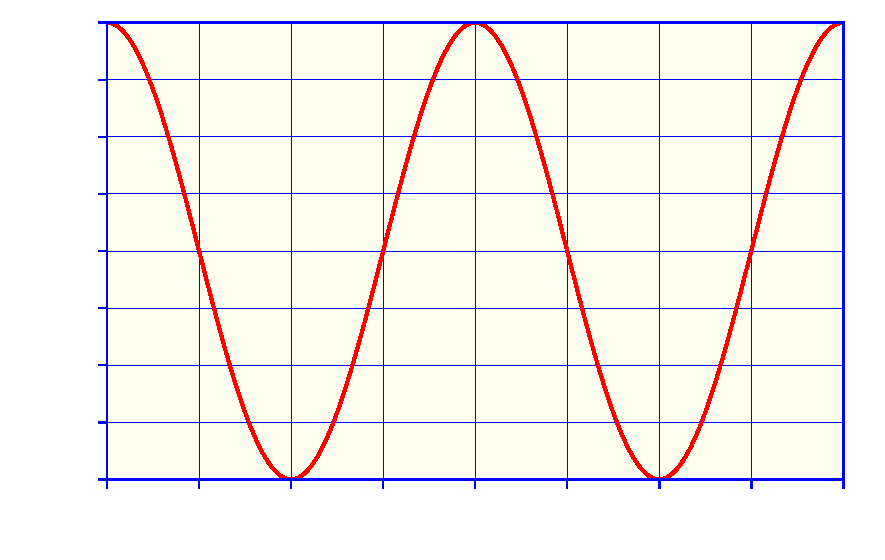
\includegraphics[width={425.00bp},height={269.00bp}]{Ape-Trigonometria-cos}}%
    \gplfronttext
  \end{picture}%
\endgroup

	\captionof{figure}{Funció cosinus} 
\end{center}

\vspace{5mm}
\begin{center}
	% GNUPLOT: LaTeX picture with Postscript
\begingroup
  \makeatletter
  \providecommand\color[2][]{%
    \GenericError{(gnuplot) \space\space\space\@spaces}{%
      Package color not loaded in conjunction with
      terminal option `colourtext'%
    }{See the gnuplot documentation for explanation.%
    }{Either use 'blacktext' in gnuplot or load the package
      color.sty in LaTeX.}%
    \renewcommand\color[2][]{}%
  }%
  \providecommand\includegraphics[2][]{%
    \GenericError{(gnuplot) \space\space\space\@spaces}{%
      Package graphicx or graphics not loaded%
    }{See the gnuplot documentation for explanation.%
    }{The gnuplot epslatex terminal needs graphicx.sty or graphics.sty.}%
    \renewcommand\includegraphics[2][]{}%
  }%
  \providecommand\rotatebox[2]{#2}%
  \@ifundefined{ifGPcolor}{%
    \newif\ifGPcolor
    \GPcolortrue
  }{}%
  \@ifundefined{ifGPblacktext}{%
    \newif\ifGPblacktext
    \GPblacktexttrue
  }{}%
  % define a \g@addto@macro without @ in the name:
  \let\gplgaddtomacro\g@addto@macro
  % define empty templates for all commands taking text:
  \gdef\gplbacktext{}%
  \gdef\gplfronttext{}%
  \makeatother
  \ifGPblacktext
    % no textcolor at all
    \def\colorrgb#1{}%
    \def\colorgray#1{}%
  \else
    % gray or color?
    \ifGPcolor
      \def\colorrgb#1{\color[rgb]{#1}}%
      \def\colorgray#1{\color[gray]{#1}}%
      \expandafter\def\csname LTw\endcsname{\color{white}}%
      \expandafter\def\csname LTb\endcsname{\color{black}}%
      \expandafter\def\csname LTa\endcsname{\color{black}}%
      \expandafter\def\csname LT0\endcsname{\color[rgb]{1,0,0}}%
      \expandafter\def\csname LT1\endcsname{\color[rgb]{0,1,0}}%
      \expandafter\def\csname LT2\endcsname{\color[rgb]{0,0,1}}%
      \expandafter\def\csname LT3\endcsname{\color[rgb]{1,0,1}}%
      \expandafter\def\csname LT4\endcsname{\color[rgb]{0,1,1}}%
      \expandafter\def\csname LT5\endcsname{\color[rgb]{1,1,0}}%
      \expandafter\def\csname LT6\endcsname{\color[rgb]{0,0,0}}%
      \expandafter\def\csname LT7\endcsname{\color[rgb]{1,0.3,0}}%
      \expandafter\def\csname LT8\endcsname{\color[rgb]{0.5,0.5,0.5}}%
    \else
      % gray
      \def\colorrgb#1{\color{black}}%
      \def\colorgray#1{\color[gray]{#1}}%
      \expandafter\def\csname LTw\endcsname{\color{white}}%
      \expandafter\def\csname LTb\endcsname{\color{black}}%
      \expandafter\def\csname LTa\endcsname{\color{black}}%
      \expandafter\def\csname LT0\endcsname{\color{black}}%
      \expandafter\def\csname LT1\endcsname{\color{black}}%
      \expandafter\def\csname LT2\endcsname{\color{black}}%
      \expandafter\def\csname LT3\endcsname{\color{black}}%
      \expandafter\def\csname LT4\endcsname{\color{black}}%
      \expandafter\def\csname LT5\endcsname{\color{black}}%
      \expandafter\def\csname LT6\endcsname{\color{black}}%
      \expandafter\def\csname LT7\endcsname{\color{black}}%
      \expandafter\def\csname LT8\endcsname{\color{black}}%
    \fi
  \fi
    \setlength{\unitlength}{0.0500bp}%
    \ifx\gptboxheight\undefined%
      \newlength{\gptboxheight}%
      \newlength{\gptboxwidth}%
      \newsavebox{\gptboxtext}%
    \fi%
    \setlength{\fboxrule}{0.5pt}%
    \setlength{\fboxsep}{1pt}%
    \definecolor{tbcol}{rgb}{1,1,1}%
\begin{picture}(8500.00,5380.00)%
    \gplgaddtomacro\gplbacktext{%
      \colorrgb{0.00,0.00,0.00}%%
      \put(548,764){\makebox(0,0)[r]{\strut{}-5}}%
      \colorrgb{0.00,0.00,0.00}%%
      \put(548,1202){\makebox(0,0)[r]{\strut{}-4}}%
      \colorrgb{0.00,0.00,0.00}%%
      \put(548,1641){\makebox(0,0)[r]{\strut{}-3}}%
      \colorrgb{0.00,0.00,0.00}%%
      \put(548,2079){\makebox(0,0)[r]{\strut{}-2}}%
      \colorrgb{0.00,0.00,0.00}%%
      \put(548,2517){\makebox(0,0)[r]{\strut{}-1}}%
      \colorrgb{0.00,0.00,0.00}%%
      \put(548,2956){\makebox(0,0)[r]{\strut{} 0}}%
      \colorrgb{0.00,0.00,0.00}%%
      \put(548,3394){\makebox(0,0)[r]{\strut{} 1}}%
      \colorrgb{0.00,0.00,0.00}%%
      \put(548,3832){\makebox(0,0)[r]{\strut{} 2}}%
      \colorrgb{0.00,0.00,0.00}%%
      \put(548,4270){\makebox(0,0)[r]{\strut{} 3}}%
      \colorrgb{0.00,0.00,0.00}%%
      \put(548,4709){\makebox(0,0)[r]{\strut{} 4}}%
      \colorrgb{0.00,0.00,0.00}%%
      \put(548,5147){\makebox(0,0)[r]{\strut{} 5}}%
      \colorrgb{0.00,0.00,0.00}%%
      \put(729,467){\makebox(0,0){\strut{}-$2\pi$}}%
      \colorrgb{0.00,0.00,0.00}%%
      \put(1649,467){\makebox(0,0){\strut{}-$\frac{3\pi}{2}$}}%
      \colorrgb{0.00,0.00,0.00}%%
      \put(2568,467){\makebox(0,0){\strut{}-$\pi$}}%
      \colorrgb{0.00,0.00,0.00}%%
      \put(3488,467){\makebox(0,0){\strut{}-$\frac{\pi}{2}$}}%
      \colorrgb{0.00,0.00,0.00}%%
      \put(4407,467){\makebox(0,0){\strut{}$0$}}%
      \colorrgb{0.00,0.00,0.00}%%
      \put(5327,467){\makebox(0,0){\strut{}$\frac{\pi}{2}$}}%
      \colorrgb{0.00,0.00,0.00}%%
      \put(6246,467){\makebox(0,0){\strut{}$\pi$}}%
      \colorrgb{0.00,0.00,0.00}%%
      \put(7165,467){\makebox(0,0){\strut{}$\frac{3\pi}{2}$}}%
      \colorrgb{0.00,0.00,0.00}%%
      \put(8085,467){\makebox(0,0){\strut{}$2\pi$}}%
    }%
    \gplgaddtomacro\gplfronttext{%
      \csname LTb\endcsname%%
      \put(178,2956){\rotatebox{-270}{\makebox(0,0){\strut{}$\sec \alpha$}}}%
      \csname LTb\endcsname%%
      \put(8138,2956){\rotatebox{-270}{\makebox(0,0){\strut{}}}}%
      \csname LTb\endcsname%%
      \put(4407,148){\makebox(0,0){\strut{}$\alpha$}}%
      \csname LTb\endcsname%%
      \put(4407,5147){\makebox(0,0){\strut{}}}%
      \csname LTb\endcsname%%
      \put(4407,5147){\makebox(0,0){\strut{}}}%
    }%
    \gplbacktext
    \put(0,0){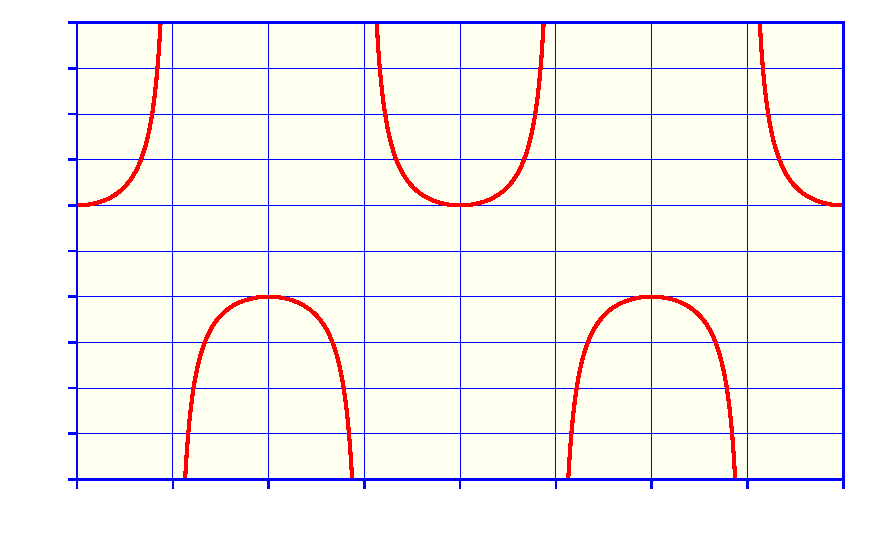
\includegraphics[width={425.00bp},height={269.00bp}]{Ape-Trigonometria-sec}}%
    \gplfronttext
  \end{picture}%
\endgroup

	\captionof{figure}{Funció secant} 
\end{center}

\begin{center}
	% GNUPLOT: LaTeX picture with Postscript
\begingroup
  \makeatletter
  \providecommand\color[2][]{%
    \GenericError{(gnuplot) \space\space\space\@spaces}{%
      Package color not loaded in conjunction with
      terminal option `colourtext'%
    }{See the gnuplot documentation for explanation.%
    }{Either use 'blacktext' in gnuplot or load the package
      color.sty in LaTeX.}%
    \renewcommand\color[2][]{}%
  }%
  \providecommand\includegraphics[2][]{%
    \GenericError{(gnuplot) \space\space\space\@spaces}{%
      Package graphicx or graphics not loaded%
    }{See the gnuplot documentation for explanation.%
    }{The gnuplot epslatex terminal needs graphicx.sty or graphics.sty.}%
    \renewcommand\includegraphics[2][]{}%
  }%
  \providecommand\rotatebox[2]{#2}%
  \@ifundefined{ifGPcolor}{%
    \newif\ifGPcolor
    \GPcolortrue
  }{}%
  \@ifundefined{ifGPblacktext}{%
    \newif\ifGPblacktext
    \GPblacktexttrue
  }{}%
  % define a \g@addto@macro without @ in the name:
  \let\gplgaddtomacro\g@addto@macro
  % define empty templates for all commands taking text:
  \gdef\gplbacktext{}%
  \gdef\gplfronttext{}%
  \makeatother
  \ifGPblacktext
    % no textcolor at all
    \def\colorrgb#1{}%
    \def\colorgray#1{}%
  \else
    % gray or color?
    \ifGPcolor
      \def\colorrgb#1{\color[rgb]{#1}}%
      \def\colorgray#1{\color[gray]{#1}}%
      \expandafter\def\csname LTw\endcsname{\color{white}}%
      \expandafter\def\csname LTb\endcsname{\color{black}}%
      \expandafter\def\csname LTa\endcsname{\color{black}}%
      \expandafter\def\csname LT0\endcsname{\color[rgb]{1,0,0}}%
      \expandafter\def\csname LT1\endcsname{\color[rgb]{0,1,0}}%
      \expandafter\def\csname LT2\endcsname{\color[rgb]{0,0,1}}%
      \expandafter\def\csname LT3\endcsname{\color[rgb]{1,0,1}}%
      \expandafter\def\csname LT4\endcsname{\color[rgb]{0,1,1}}%
      \expandafter\def\csname LT5\endcsname{\color[rgb]{1,1,0}}%
      \expandafter\def\csname LT6\endcsname{\color[rgb]{0,0,0}}%
      \expandafter\def\csname LT7\endcsname{\color[rgb]{1,0.3,0}}%
      \expandafter\def\csname LT8\endcsname{\color[rgb]{0.5,0.5,0.5}}%
    \else
      % gray
      \def\colorrgb#1{\color{black}}%
      \def\colorgray#1{\color[gray]{#1}}%
      \expandafter\def\csname LTw\endcsname{\color{white}}%
      \expandafter\def\csname LTb\endcsname{\color{black}}%
      \expandafter\def\csname LTa\endcsname{\color{black}}%
      \expandafter\def\csname LT0\endcsname{\color{black}}%
      \expandafter\def\csname LT1\endcsname{\color{black}}%
      \expandafter\def\csname LT2\endcsname{\color{black}}%
      \expandafter\def\csname LT3\endcsname{\color{black}}%
      \expandafter\def\csname LT4\endcsname{\color{black}}%
      \expandafter\def\csname LT5\endcsname{\color{black}}%
      \expandafter\def\csname LT6\endcsname{\color{black}}%
      \expandafter\def\csname LT7\endcsname{\color{black}}%
      \expandafter\def\csname LT8\endcsname{\color{black}}%
    \fi
  \fi
    \setlength{\unitlength}{0.0500bp}%
    \ifx\gptboxheight\undefined%
      \newlength{\gptboxheight}%
      \newlength{\gptboxwidth}%
      \newsavebox{\gptboxtext}%
    \fi%
    \setlength{\fboxrule}{0.5pt}%
    \setlength{\fboxsep}{1pt}%
    \definecolor{tbcol}{rgb}{1,1,1}%
\begin{picture}(8500.00,5380.00)%
    \gplgaddtomacro\gplbacktext{%
      \colorrgb{0.00,0.00,0.00}%%
      \put(644,764){\makebox(0,0)[r]{\strut{}-10}}%
      \colorrgb{0.00,0.00,0.00}%%
      \put(644,1202){\makebox(0,0)[r]{\strut{}-8}}%
      \colorrgb{0.00,0.00,0.00}%%
      \put(644,1641){\makebox(0,0)[r]{\strut{}-6}}%
      \colorrgb{0.00,0.00,0.00}%%
      \put(644,2079){\makebox(0,0)[r]{\strut{}-4}}%
      \colorrgb{0.00,0.00,0.00}%%
      \put(644,2517){\makebox(0,0)[r]{\strut{}-2}}%
      \colorrgb{0.00,0.00,0.00}%%
      \put(644,2956){\makebox(0,0)[r]{\strut{} 0}}%
      \colorrgb{0.00,0.00,0.00}%%
      \put(644,3394){\makebox(0,0)[r]{\strut{} 2}}%
      \colorrgb{0.00,0.00,0.00}%%
      \put(644,3832){\makebox(0,0)[r]{\strut{} 4}}%
      \colorrgb{0.00,0.00,0.00}%%
      \put(644,4270){\makebox(0,0)[r]{\strut{} 6}}%
      \colorrgb{0.00,0.00,0.00}%%
      \put(644,4709){\makebox(0,0)[r]{\strut{} 8}}%
      \colorrgb{0.00,0.00,0.00}%%
      \put(644,5147){\makebox(0,0)[r]{\strut{} 10}}%
      \colorrgb{0.00,0.00,0.00}%%
      \put(825,467){\makebox(0,0){\strut{}-$2\pi$}}%
      \colorrgb{0.00,0.00,0.00}%%
      \put(1733,467){\makebox(0,0){\strut{}-$\frac{3\pi}{2}$}}%
      \colorrgb{0.00,0.00,0.00}%%
      \put(2640,467){\makebox(0,0){\strut{}-$\pi$}}%
      \colorrgb{0.00,0.00,0.00}%%
      \put(3548,467){\makebox(0,0){\strut{}-$\frac{\pi}{2}$}}%
      \colorrgb{0.00,0.00,0.00}%%
      \put(4455,467){\makebox(0,0){\strut{}$0$}}%
      \colorrgb{0.00,0.00,0.00}%%
      \put(5363,467){\makebox(0,0){\strut{}$\frac{\pi}{2}$}}%
      \colorrgb{0.00,0.00,0.00}%%
      \put(6270,467){\makebox(0,0){\strut{}$\pi$}}%
      \colorrgb{0.00,0.00,0.00}%%
      \put(7178,467){\makebox(0,0){\strut{}$\frac{3\pi}{2}$}}%
      \colorrgb{0.00,0.00,0.00}%%
      \put(8085,467){\makebox(0,0){\strut{}$2\pi$}}%
    }%
    \gplgaddtomacro\gplfronttext{%
      \csname LTb\endcsname%%
      \put(178,2956){\rotatebox{-270}{\makebox(0,0){\strut{}$\tan \alpha$}}}%
      \csname LTb\endcsname%%
      \put(8138,2956){\rotatebox{-270}{\makebox(0,0){\strut{}}}}%
      \csname LTb\endcsname%%
      \put(4455,148){\makebox(0,0){\strut{}$\alpha$}}%
      \csname LTb\endcsname%%
      \put(4455,5147){\makebox(0,0){\strut{}}}%
      \csname LTb\endcsname%%
      \put(4455,5147){\makebox(0,0){\strut{}}}%
    }%
    \gplbacktext
    \put(0,0){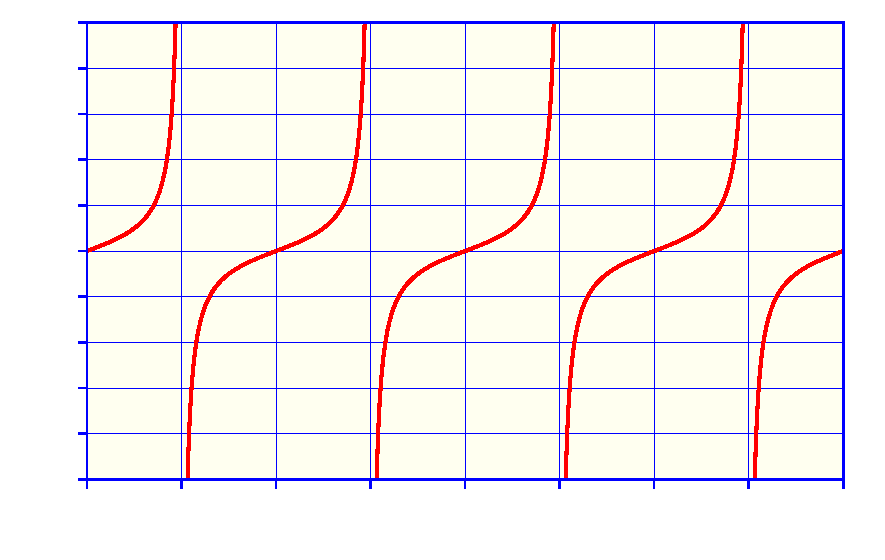
\includegraphics[width={425.00bp},height={269.00bp}]{Ape-Trigonometria-tan}}%
    \gplfronttext
  \end{picture}%
\endgroup

	\captionof{figure}{Funció tangent} 
\end{center}

\vspace{5mm}
\begin{center}
	% GNUPLOT: LaTeX picture with Postscript
\begingroup
  \makeatletter
  \providecommand\color[2][]{%
    \GenericError{(gnuplot) \space\space\space\@spaces}{%
      Package color not loaded in conjunction with
      terminal option `colourtext'%
    }{See the gnuplot documentation for explanation.%
    }{Either use 'blacktext' in gnuplot or load the package
      color.sty in LaTeX.}%
    \renewcommand\color[2][]{}%
  }%
  \providecommand\includegraphics[2][]{%
    \GenericError{(gnuplot) \space\space\space\@spaces}{%
      Package graphicx or graphics not loaded%
    }{See the gnuplot documentation for explanation.%
    }{The gnuplot epslatex terminal needs graphicx.sty or graphics.sty.}%
    \renewcommand\includegraphics[2][]{}%
  }%
  \providecommand\rotatebox[2]{#2}%
  \@ifundefined{ifGPcolor}{%
    \newif\ifGPcolor
    \GPcolortrue
  }{}%
  \@ifundefined{ifGPblacktext}{%
    \newif\ifGPblacktext
    \GPblacktexttrue
  }{}%
  % define a \g@addto@macro without @ in the name:
  \let\gplgaddtomacro\g@addto@macro
  % define empty templates for all commands taking text:
  \gdef\gplbacktext{}%
  \gdef\gplfronttext{}%
  \makeatother
  \ifGPblacktext
    % no textcolor at all
    \def\colorrgb#1{}%
    \def\colorgray#1{}%
  \else
    % gray or color?
    \ifGPcolor
      \def\colorrgb#1{\color[rgb]{#1}}%
      \def\colorgray#1{\color[gray]{#1}}%
      \expandafter\def\csname LTw\endcsname{\color{white}}%
      \expandafter\def\csname LTb\endcsname{\color{black}}%
      \expandafter\def\csname LTa\endcsname{\color{black}}%
      \expandafter\def\csname LT0\endcsname{\color[rgb]{1,0,0}}%
      \expandafter\def\csname LT1\endcsname{\color[rgb]{0,1,0}}%
      \expandafter\def\csname LT2\endcsname{\color[rgb]{0,0,1}}%
      \expandafter\def\csname LT3\endcsname{\color[rgb]{1,0,1}}%
      \expandafter\def\csname LT4\endcsname{\color[rgb]{0,1,1}}%
      \expandafter\def\csname LT5\endcsname{\color[rgb]{1,1,0}}%
      \expandafter\def\csname LT6\endcsname{\color[rgb]{0,0,0}}%
      \expandafter\def\csname LT7\endcsname{\color[rgb]{1,0.3,0}}%
      \expandafter\def\csname LT8\endcsname{\color[rgb]{0.5,0.5,0.5}}%
    \else
      % gray
      \def\colorrgb#1{\color{black}}%
      \def\colorgray#1{\color[gray]{#1}}%
      \expandafter\def\csname LTw\endcsname{\color{white}}%
      \expandafter\def\csname LTb\endcsname{\color{black}}%
      \expandafter\def\csname LTa\endcsname{\color{black}}%
      \expandafter\def\csname LT0\endcsname{\color{black}}%
      \expandafter\def\csname LT1\endcsname{\color{black}}%
      \expandafter\def\csname LT2\endcsname{\color{black}}%
      \expandafter\def\csname LT3\endcsname{\color{black}}%
      \expandafter\def\csname LT4\endcsname{\color{black}}%
      \expandafter\def\csname LT5\endcsname{\color{black}}%
      \expandafter\def\csname LT6\endcsname{\color{black}}%
      \expandafter\def\csname LT7\endcsname{\color{black}}%
      \expandafter\def\csname LT8\endcsname{\color{black}}%
    \fi
  \fi
    \setlength{\unitlength}{0.0500bp}%
    \ifx\gptboxheight\undefined%
      \newlength{\gptboxheight}%
      \newlength{\gptboxwidth}%
      \newsavebox{\gptboxtext}%
    \fi%
    \setlength{\fboxrule}{0.5pt}%
    \setlength{\fboxsep}{1pt}%
    \definecolor{tbcol}{rgb}{1,1,1}%
\begin{picture}(8500.00,5380.00)%
    \gplgaddtomacro\gplbacktext{%
      \colorrgb{0.00,0.00,0.00}%%
      \put(644,764){\makebox(0,0)[r]{\strut{}-10}}%
      \colorrgb{0.00,0.00,0.00}%%
      \put(644,1202){\makebox(0,0)[r]{\strut{}-8}}%
      \colorrgb{0.00,0.00,0.00}%%
      \put(644,1641){\makebox(0,0)[r]{\strut{}-6}}%
      \colorrgb{0.00,0.00,0.00}%%
      \put(644,2079){\makebox(0,0)[r]{\strut{}-4}}%
      \colorrgb{0.00,0.00,0.00}%%
      \put(644,2517){\makebox(0,0)[r]{\strut{}-2}}%
      \colorrgb{0.00,0.00,0.00}%%
      \put(644,2956){\makebox(0,0)[r]{\strut{} 0}}%
      \colorrgb{0.00,0.00,0.00}%%
      \put(644,3394){\makebox(0,0)[r]{\strut{} 2}}%
      \colorrgb{0.00,0.00,0.00}%%
      \put(644,3832){\makebox(0,0)[r]{\strut{} 4}}%
      \colorrgb{0.00,0.00,0.00}%%
      \put(644,4270){\makebox(0,0)[r]{\strut{} 6}}%
      \colorrgb{0.00,0.00,0.00}%%
      \put(644,4709){\makebox(0,0)[r]{\strut{} 8}}%
      \colorrgb{0.00,0.00,0.00}%%
      \put(644,5147){\makebox(0,0)[r]{\strut{} 10}}%
      \colorrgb{0.00,0.00,0.00}%%
      \put(825,467){\makebox(0,0){\strut{}-$2\pi$}}%
      \colorrgb{0.00,0.00,0.00}%%
      \put(1733,467){\makebox(0,0){\strut{}-$\frac{3\pi}{2}$}}%
      \colorrgb{0.00,0.00,0.00}%%
      \put(2640,467){\makebox(0,0){\strut{}-$\pi$}}%
      \colorrgb{0.00,0.00,0.00}%%
      \put(3548,467){\makebox(0,0){\strut{}-$\frac{\pi}{2}$}}%
      \colorrgb{0.00,0.00,0.00}%%
      \put(4455,467){\makebox(0,0){\strut{}$0$}}%
      \colorrgb{0.00,0.00,0.00}%%
      \put(5363,467){\makebox(0,0){\strut{}$\frac{\pi}{2}$}}%
      \colorrgb{0.00,0.00,0.00}%%
      \put(6270,467){\makebox(0,0){\strut{}$\pi$}}%
      \colorrgb{0.00,0.00,0.00}%%
      \put(7178,467){\makebox(0,0){\strut{}$\frac{3\pi}{2}$}}%
      \colorrgb{0.00,0.00,0.00}%%
      \put(8085,467){\makebox(0,0){\strut{}$2\pi$}}%
    }%
    \gplgaddtomacro\gplfronttext{%
      \csname LTb\endcsname%%
      \put(178,2956){\rotatebox{-270}{\makebox(0,0){\strut{}$\cot \alpha$}}}%
      \csname LTb\endcsname%%
      \put(8138,2956){\rotatebox{-270}{\makebox(0,0){\strut{}}}}%
      \csname LTb\endcsname%%
      \put(4455,148){\makebox(0,0){\strut{}$\alpha$}}%
      \csname LTb\endcsname%%
      \put(4455,5147){\makebox(0,0){\strut{}}}%
      \csname LTb\endcsname%%
      \put(4455,5147){\makebox(0,0){\strut{}}}%
    }%
    \gplbacktext
    \put(0,0){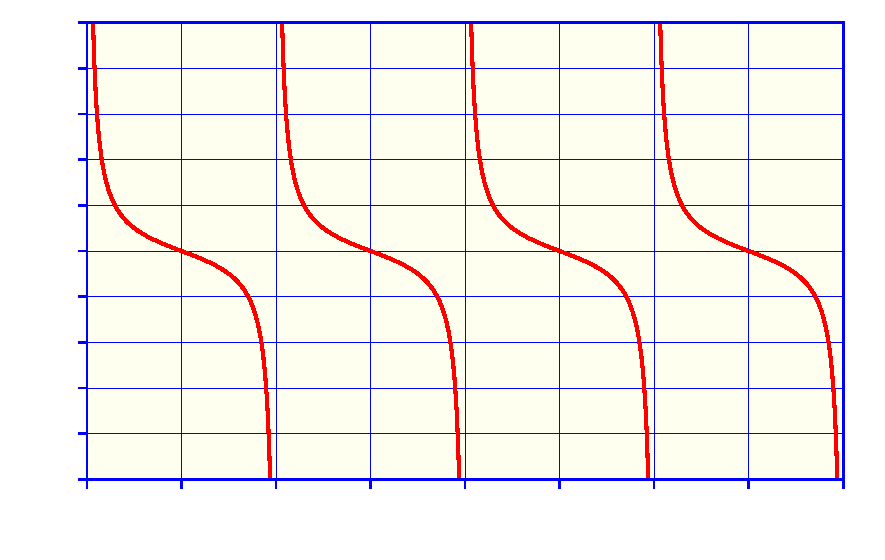
\includegraphics[width={425.00bp},height={269.00bp}]{Ape-Trigonometria-cot}}%
    \gplfronttext
  \end{picture}%
\endgroup

	\captionof{figure}{Funció cotangent} 
\end{center}

\begin{center}
	% GNUPLOT: LaTeX picture with Postscript
\begingroup
  \makeatletter
  \providecommand\color[2][]{%
    \GenericError{(gnuplot) \space\space\space\@spaces}{%
      Package color not loaded in conjunction with
      terminal option `colourtext'%
    }{See the gnuplot documentation for explanation.%
    }{Either use 'blacktext' in gnuplot or load the package
      color.sty in LaTeX.}%
    \renewcommand\color[2][]{}%
  }%
  \providecommand\includegraphics[2][]{%
    \GenericError{(gnuplot) \space\space\space\@spaces}{%
      Package graphicx or graphics not loaded%
    }{See the gnuplot documentation for explanation.%
    }{The gnuplot epslatex terminal needs graphicx.sty or graphics.sty.}%
    \renewcommand\includegraphics[2][]{}%
  }%
  \providecommand\rotatebox[2]{#2}%
  \@ifundefined{ifGPcolor}{%
    \newif\ifGPcolor
    \GPcolortrue
  }{}%
  \@ifundefined{ifGPblacktext}{%
    \newif\ifGPblacktext
    \GPblacktexttrue
  }{}%
  % define a \g@addto@macro without @ in the name:
  \let\gplgaddtomacro\g@addto@macro
  % define empty templates for all commands taking text:
  \gdef\gplbacktext{}%
  \gdef\gplfronttext{}%
  \makeatother
  \ifGPblacktext
    % no textcolor at all
    \def\colorrgb#1{}%
    \def\colorgray#1{}%
  \else
    % gray or color?
    \ifGPcolor
      \def\colorrgb#1{\color[rgb]{#1}}%
      \def\colorgray#1{\color[gray]{#1}}%
      \expandafter\def\csname LTw\endcsname{\color{white}}%
      \expandafter\def\csname LTb\endcsname{\color{black}}%
      \expandafter\def\csname LTa\endcsname{\color{black}}%
      \expandafter\def\csname LT0\endcsname{\color[rgb]{1,0,0}}%
      \expandafter\def\csname LT1\endcsname{\color[rgb]{0,1,0}}%
      \expandafter\def\csname LT2\endcsname{\color[rgb]{0,0,1}}%
      \expandafter\def\csname LT3\endcsname{\color[rgb]{1,0,1}}%
      \expandafter\def\csname LT4\endcsname{\color[rgb]{0,1,1}}%
      \expandafter\def\csname LT5\endcsname{\color[rgb]{1,1,0}}%
      \expandafter\def\csname LT6\endcsname{\color[rgb]{0,0,0}}%
      \expandafter\def\csname LT7\endcsname{\color[rgb]{1,0.3,0}}%
      \expandafter\def\csname LT8\endcsname{\color[rgb]{0.5,0.5,0.5}}%
    \else
      % gray
      \def\colorrgb#1{\color{black}}%
      \def\colorgray#1{\color[gray]{#1}}%
      \expandafter\def\csname LTw\endcsname{\color{white}}%
      \expandafter\def\csname LTb\endcsname{\color{black}}%
      \expandafter\def\csname LTa\endcsname{\color{black}}%
      \expandafter\def\csname LT0\endcsname{\color{black}}%
      \expandafter\def\csname LT1\endcsname{\color{black}}%
      \expandafter\def\csname LT2\endcsname{\color{black}}%
      \expandafter\def\csname LT3\endcsname{\color{black}}%
      \expandafter\def\csname LT4\endcsname{\color{black}}%
      \expandafter\def\csname LT5\endcsname{\color{black}}%
      \expandafter\def\csname LT6\endcsname{\color{black}}%
      \expandafter\def\csname LT7\endcsname{\color{black}}%
      \expandafter\def\csname LT8\endcsname{\color{black}}%
    \fi
  \fi
    \setlength{\unitlength}{0.0500bp}%
    \ifx\gptboxheight\undefined%
      \newlength{\gptboxheight}%
      \newlength{\gptboxwidth}%
      \newsavebox{\gptboxtext}%
    \fi%
    \setlength{\fboxrule}{0.5pt}%
    \setlength{\fboxsep}{1pt}%
    \definecolor{tbcol}{rgb}{1,1,1}%
\begin{picture}(8500.00,5380.00)%
    \gplgaddtomacro\gplbacktext{%
      \colorrgb{0.00,0.00,0.00}%%
      \put(644,764){\makebox(0,0)[r]{\strut{}-80}}%
      \colorrgb{0.00,0.00,0.00}%%
      \put(644,1312){\makebox(0,0)[r]{\strut{}-60}}%
      \colorrgb{0.00,0.00,0.00}%%
      \put(644,1860){\makebox(0,0)[r]{\strut{}-40}}%
      \colorrgb{0.00,0.00,0.00}%%
      \put(644,2408){\makebox(0,0)[r]{\strut{}-20}}%
      \colorrgb{0.00,0.00,0.00}%%
      \put(644,2956){\makebox(0,0)[r]{\strut{} 0}}%
      \colorrgb{0.00,0.00,0.00}%%
      \put(644,3503){\makebox(0,0)[r]{\strut{} 20}}%
      \colorrgb{0.00,0.00,0.00}%%
      \put(644,4051){\makebox(0,0)[r]{\strut{} 40}}%
      \colorrgb{0.00,0.00,0.00}%%
      \put(644,4599){\makebox(0,0)[r]{\strut{} 60}}%
      \colorrgb{0.00,0.00,0.00}%%
      \put(644,5147){\makebox(0,0)[r]{\strut{} 80}}%
      \colorrgb{0.00,0.00,0.00}%%
      \put(825,467){\makebox(0,0){\strut{}-5}}%
      \colorrgb{0.00,0.00,0.00}%%
      \put(1551,467){\makebox(0,0){\strut{}-4}}%
      \colorrgb{0.00,0.00,0.00}%%
      \put(2277,467){\makebox(0,0){\strut{}-3}}%
      \colorrgb{0.00,0.00,0.00}%%
      \put(3003,467){\makebox(0,0){\strut{}-2}}%
      \colorrgb{0.00,0.00,0.00}%%
      \put(3729,467){\makebox(0,0){\strut{}-1}}%
      \colorrgb{0.00,0.00,0.00}%%
      \put(4455,467){\makebox(0,0){\strut{} 0}}%
      \colorrgb{0.00,0.00,0.00}%%
      \put(5181,467){\makebox(0,0){\strut{} 1}}%
      \colorrgb{0.00,0.00,0.00}%%
      \put(5907,467){\makebox(0,0){\strut{} 2}}%
      \colorrgb{0.00,0.00,0.00}%%
      \put(6633,467){\makebox(0,0){\strut{} 3}}%
      \colorrgb{0.00,0.00,0.00}%%
      \put(7359,467){\makebox(0,0){\strut{} 4}}%
      \colorrgb{0.00,0.00,0.00}%%
      \put(8085,467){\makebox(0,0){\strut{} 5}}%
    }%
    \gplgaddtomacro\gplfronttext{%
      \csname LTb\endcsname%%
      \put(178,2956){\rotatebox{-270}{\makebox(0,0){\strut{}$\sinh z$}}}%
      \csname LTb\endcsname%%
      \put(8138,2956){\rotatebox{-270}{\makebox(0,0){\strut{}}}}%
      \csname LTb\endcsname%%
      \put(4455,148){\makebox(0,0){\strut{}$z$}}%
      \csname LTb\endcsname%%
      \put(4455,5147){\makebox(0,0){\strut{}}}%
      \csname LTb\endcsname%%
      \put(4455,5147){\makebox(0,0){\strut{}}}%
    }%
    \gplbacktext
    \put(0,0){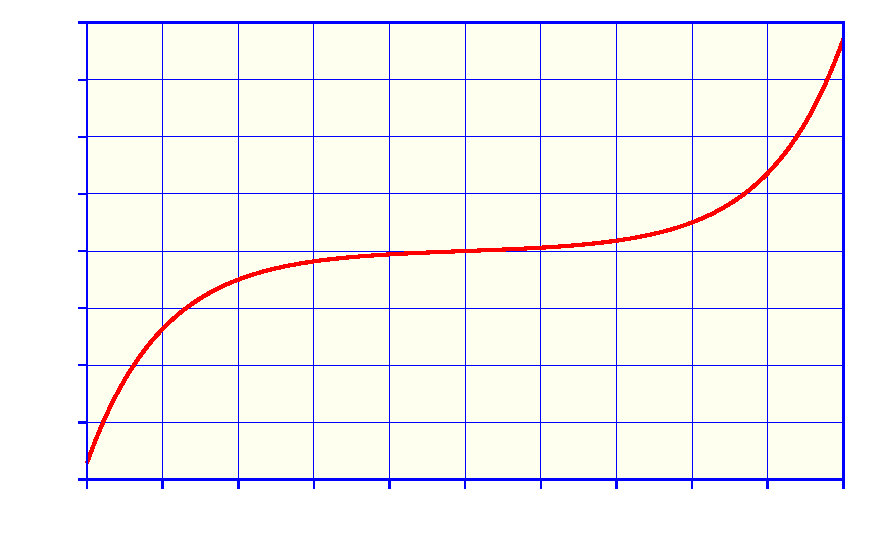
\includegraphics[width={425.00bp},height={269.00bp}]{Ape-Trigonometria-sinh}}%
    \gplfronttext
  \end{picture}%
\endgroup

	\captionof{figure}{Funció sinus hiperbòlic} 
\end{center}

\begin{center}
	% GNUPLOT: LaTeX picture with Postscript
\begingroup
  \makeatletter
  \providecommand\color[2][]{%
    \GenericError{(gnuplot) \space\space\space\@spaces}{%
      Package color not loaded in conjunction with
      terminal option `colourtext'%
    }{See the gnuplot documentation for explanation.%
    }{Either use 'blacktext' in gnuplot or load the package
      color.sty in LaTeX.}%
    \renewcommand\color[2][]{}%
  }%
  \providecommand\includegraphics[2][]{%
    \GenericError{(gnuplot) \space\space\space\@spaces}{%
      Package graphicx or graphics not loaded%
    }{See the gnuplot documentation for explanation.%
    }{The gnuplot epslatex terminal needs graphicx.sty or graphics.sty.}%
    \renewcommand\includegraphics[2][]{}%
  }%
  \providecommand\rotatebox[2]{#2}%
  \@ifundefined{ifGPcolor}{%
    \newif\ifGPcolor
    \GPcolortrue
  }{}%
  \@ifundefined{ifGPblacktext}{%
    \newif\ifGPblacktext
    \GPblacktexttrue
  }{}%
  % define a \g@addto@macro without @ in the name:
  \let\gplgaddtomacro\g@addto@macro
  % define empty templates for all commands taking text:
  \gdef\gplbacktext{}%
  \gdef\gplfronttext{}%
  \makeatother
  \ifGPblacktext
    % no textcolor at all
    \def\colorrgb#1{}%
    \def\colorgray#1{}%
  \else
    % gray or color?
    \ifGPcolor
      \def\colorrgb#1{\color[rgb]{#1}}%
      \def\colorgray#1{\color[gray]{#1}}%
      \expandafter\def\csname LTw\endcsname{\color{white}}%
      \expandafter\def\csname LTb\endcsname{\color{black}}%
      \expandafter\def\csname LTa\endcsname{\color{black}}%
      \expandafter\def\csname LT0\endcsname{\color[rgb]{1,0,0}}%
      \expandafter\def\csname LT1\endcsname{\color[rgb]{0,1,0}}%
      \expandafter\def\csname LT2\endcsname{\color[rgb]{0,0,1}}%
      \expandafter\def\csname LT3\endcsname{\color[rgb]{1,0,1}}%
      \expandafter\def\csname LT4\endcsname{\color[rgb]{0,1,1}}%
      \expandafter\def\csname LT5\endcsname{\color[rgb]{1,1,0}}%
      \expandafter\def\csname LT6\endcsname{\color[rgb]{0,0,0}}%
      \expandafter\def\csname LT7\endcsname{\color[rgb]{1,0.3,0}}%
      \expandafter\def\csname LT8\endcsname{\color[rgb]{0.5,0.5,0.5}}%
    \else
      % gray
      \def\colorrgb#1{\color{black}}%
      \def\colorgray#1{\color[gray]{#1}}%
      \expandafter\def\csname LTw\endcsname{\color{white}}%
      \expandafter\def\csname LTb\endcsname{\color{black}}%
      \expandafter\def\csname LTa\endcsname{\color{black}}%
      \expandafter\def\csname LT0\endcsname{\color{black}}%
      \expandafter\def\csname LT1\endcsname{\color{black}}%
      \expandafter\def\csname LT2\endcsname{\color{black}}%
      \expandafter\def\csname LT3\endcsname{\color{black}}%
      \expandafter\def\csname LT4\endcsname{\color{black}}%
      \expandafter\def\csname LT5\endcsname{\color{black}}%
      \expandafter\def\csname LT6\endcsname{\color{black}}%
      \expandafter\def\csname LT7\endcsname{\color{black}}%
      \expandafter\def\csname LT8\endcsname{\color{black}}%
    \fi
  \fi
    \setlength{\unitlength}{0.0500bp}%
    \ifx\gptboxheight\undefined%
      \newlength{\gptboxheight}%
      \newlength{\gptboxwidth}%
      \newsavebox{\gptboxtext}%
    \fi%
    \setlength{\fboxrule}{0.5pt}%
    \setlength{\fboxsep}{1pt}%
    \definecolor{tbcol}{rgb}{1,1,1}%
\begin{picture}(8500.00,5380.00)%
    \gplgaddtomacro\gplbacktext{%
      \colorrgb{0.00,0.00,0.00}%%
      \put(548,764){\makebox(0,0)[r]{\strut{}-5}}%
      \colorrgb{0.00,0.00,0.00}%%
      \put(548,1202){\makebox(0,0)[r]{\strut{}-4}}%
      \colorrgb{0.00,0.00,0.00}%%
      \put(548,1641){\makebox(0,0)[r]{\strut{}-3}}%
      \colorrgb{0.00,0.00,0.00}%%
      \put(548,2079){\makebox(0,0)[r]{\strut{}-2}}%
      \colorrgb{0.00,0.00,0.00}%%
      \put(548,2517){\makebox(0,0)[r]{\strut{}-1}}%
      \colorrgb{0.00,0.00,0.00}%%
      \put(548,2956){\makebox(0,0)[r]{\strut{} 0}}%
      \colorrgb{0.00,0.00,0.00}%%
      \put(548,3394){\makebox(0,0)[r]{\strut{} 1}}%
      \colorrgb{0.00,0.00,0.00}%%
      \put(548,3832){\makebox(0,0)[r]{\strut{} 2}}%
      \colorrgb{0.00,0.00,0.00}%%
      \put(548,4270){\makebox(0,0)[r]{\strut{} 3}}%
      \colorrgb{0.00,0.00,0.00}%%
      \put(548,4709){\makebox(0,0)[r]{\strut{} 4}}%
      \colorrgb{0.00,0.00,0.00}%%
      \put(548,5147){\makebox(0,0)[r]{\strut{} 5}}%
      \colorrgb{0.00,0.00,0.00}%%
      \put(729,467){\makebox(0,0){\strut{}-5}}%
      \colorrgb{0.00,0.00,0.00}%%
      \put(1465,467){\makebox(0,0){\strut{}-4}}%
      \colorrgb{0.00,0.00,0.00}%%
      \put(2200,467){\makebox(0,0){\strut{}-3}}%
      \colorrgb{0.00,0.00,0.00}%%
      \put(2936,467){\makebox(0,0){\strut{}-2}}%
      \colorrgb{0.00,0.00,0.00}%%
      \put(3672,467){\makebox(0,0){\strut{}-1}}%
      \colorrgb{0.00,0.00,0.00}%%
      \put(4407,467){\makebox(0,0){\strut{} 0}}%
      \colorrgb{0.00,0.00,0.00}%%
      \put(5143,467){\makebox(0,0){\strut{} 1}}%
      \colorrgb{0.00,0.00,0.00}%%
      \put(5878,467){\makebox(0,0){\strut{} 2}}%
      \colorrgb{0.00,0.00,0.00}%%
      \put(6614,467){\makebox(0,0){\strut{} 3}}%
      \colorrgb{0.00,0.00,0.00}%%
      \put(7349,467){\makebox(0,0){\strut{} 4}}%
      \colorrgb{0.00,0.00,0.00}%%
      \put(8085,467){\makebox(0,0){\strut{} 5}}%
    }%
    \gplgaddtomacro\gplfronttext{%
      \csname LTb\endcsname%%
      \put(178,2956){\rotatebox{-270}{\makebox(0,0){\strut{}$\csch z$}}}%
      \csname LTb\endcsname%%
      \put(8138,2956){\rotatebox{-270}{\makebox(0,0){\strut{}}}}%
      \csname LTb\endcsname%%
      \put(4407,148){\makebox(0,0){\strut{}$z$}}%
      \csname LTb\endcsname%%
      \put(4407,5147){\makebox(0,0){\strut{}}}%
      \csname LTb\endcsname%%
      \put(4407,5147){\makebox(0,0){\strut{}}}%
    }%
    \gplbacktext
    \put(0,0){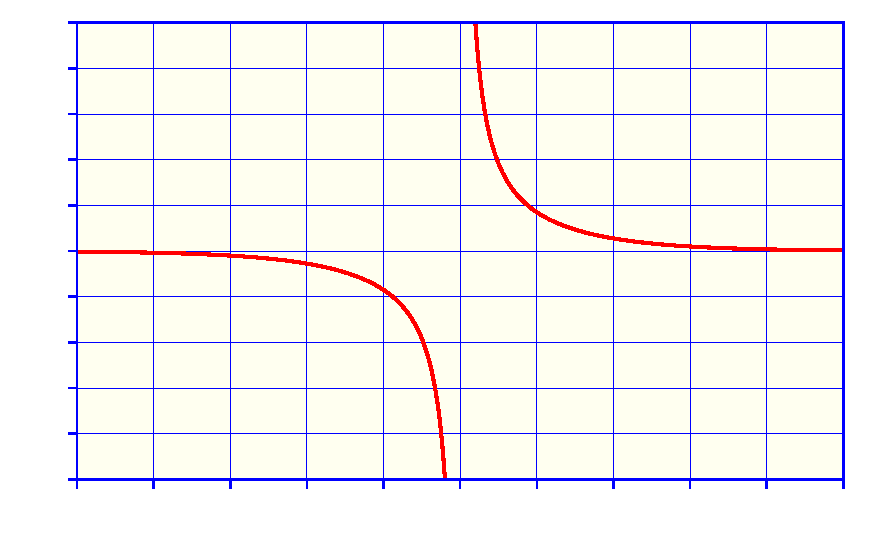
\includegraphics[width={425.00bp},height={269.00bp}]{Ape-Trigonometria-csch}}%
    \gplfronttext
  \end{picture}%
\endgroup

	\captionof{figure}{Funció cosecant hiperbòlica} 
\end{center}

\vspace{5mm}
\begin{center}
	% GNUPLOT: LaTeX picture with Postscript
\begingroup
  \makeatletter
  \providecommand\color[2][]{%
    \GenericError{(gnuplot) \space\space\space\@spaces}{%
      Package color not loaded in conjunction with
      terminal option `colourtext'%
    }{See the gnuplot documentation for explanation.%
    }{Either use 'blacktext' in gnuplot or load the package
      color.sty in LaTeX.}%
    \renewcommand\color[2][]{}%
  }%
  \providecommand\includegraphics[2][]{%
    \GenericError{(gnuplot) \space\space\space\@spaces}{%
      Package graphicx or graphics not loaded%
    }{See the gnuplot documentation for explanation.%
    }{The gnuplot epslatex terminal needs graphicx.sty or graphics.sty.}%
    \renewcommand\includegraphics[2][]{}%
  }%
  \providecommand\rotatebox[2]{#2}%
  \@ifundefined{ifGPcolor}{%
    \newif\ifGPcolor
    \GPcolortrue
  }{}%
  \@ifundefined{ifGPblacktext}{%
    \newif\ifGPblacktext
    \GPblacktexttrue
  }{}%
  % define a \g@addto@macro without @ in the name:
  \let\gplgaddtomacro\g@addto@macro
  % define empty templates for all commands taking text:
  \gdef\gplbacktext{}%
  \gdef\gplfronttext{}%
  \makeatother
  \ifGPblacktext
    % no textcolor at all
    \def\colorrgb#1{}%
    \def\colorgray#1{}%
  \else
    % gray or color?
    \ifGPcolor
      \def\colorrgb#1{\color[rgb]{#1}}%
      \def\colorgray#1{\color[gray]{#1}}%
      \expandafter\def\csname LTw\endcsname{\color{white}}%
      \expandafter\def\csname LTb\endcsname{\color{black}}%
      \expandafter\def\csname LTa\endcsname{\color{black}}%
      \expandafter\def\csname LT0\endcsname{\color[rgb]{1,0,0}}%
      \expandafter\def\csname LT1\endcsname{\color[rgb]{0,1,0}}%
      \expandafter\def\csname LT2\endcsname{\color[rgb]{0,0,1}}%
      \expandafter\def\csname LT3\endcsname{\color[rgb]{1,0,1}}%
      \expandafter\def\csname LT4\endcsname{\color[rgb]{0,1,1}}%
      \expandafter\def\csname LT5\endcsname{\color[rgb]{1,1,0}}%
      \expandafter\def\csname LT6\endcsname{\color[rgb]{0,0,0}}%
      \expandafter\def\csname LT7\endcsname{\color[rgb]{1,0.3,0}}%
      \expandafter\def\csname LT8\endcsname{\color[rgb]{0.5,0.5,0.5}}%
    \else
      % gray
      \def\colorrgb#1{\color{black}}%
      \def\colorgray#1{\color[gray]{#1}}%
      \expandafter\def\csname LTw\endcsname{\color{white}}%
      \expandafter\def\csname LTb\endcsname{\color{black}}%
      \expandafter\def\csname LTa\endcsname{\color{black}}%
      \expandafter\def\csname LT0\endcsname{\color{black}}%
      \expandafter\def\csname LT1\endcsname{\color{black}}%
      \expandafter\def\csname LT2\endcsname{\color{black}}%
      \expandafter\def\csname LT3\endcsname{\color{black}}%
      \expandafter\def\csname LT4\endcsname{\color{black}}%
      \expandafter\def\csname LT5\endcsname{\color{black}}%
      \expandafter\def\csname LT6\endcsname{\color{black}}%
      \expandafter\def\csname LT7\endcsname{\color{black}}%
      \expandafter\def\csname LT8\endcsname{\color{black}}%
    \fi
  \fi
    \setlength{\unitlength}{0.0500bp}%
    \ifx\gptboxheight\undefined%
      \newlength{\gptboxheight}%
      \newlength{\gptboxwidth}%
      \newsavebox{\gptboxtext}%
    \fi%
    \setlength{\fboxrule}{0.5pt}%
    \setlength{\fboxsep}{1pt}%
    \definecolor{tbcol}{rgb}{1,1,1}%
\begin{picture}(8500.00,5380.00)%
    \gplgaddtomacro\gplbacktext{%
      \colorrgb{0.00,0.00,0.00}%%
      \put(548,764){\makebox(0,0)[r]{\strut{}$0$}}%
      \colorrgb{0.00,0.00,0.00}%%
      \put(548,1312){\makebox(0,0)[r]{\strut{}$10$}}%
      \colorrgb{0.00,0.00,0.00}%%
      \put(548,1860){\makebox(0,0)[r]{\strut{}$20$}}%
      \colorrgb{0.00,0.00,0.00}%%
      \put(548,2408){\makebox(0,0)[r]{\strut{}$30$}}%
      \colorrgb{0.00,0.00,0.00}%%
      \put(548,2956){\makebox(0,0)[r]{\strut{}$40$}}%
      \colorrgb{0.00,0.00,0.00}%%
      \put(548,3503){\makebox(0,0)[r]{\strut{}$50$}}%
      \colorrgb{0.00,0.00,0.00}%%
      \put(548,4051){\makebox(0,0)[r]{\strut{}$60$}}%
      \colorrgb{0.00,0.00,0.00}%%
      \put(548,4599){\makebox(0,0)[r]{\strut{}$70$}}%
      \colorrgb{0.00,0.00,0.00}%%
      \put(548,5147){\makebox(0,0)[r]{\strut{}$80$}}%
      \colorrgb{0.00,0.00,0.00}%%
      \put(729,467){\makebox(0,0){\strut{}-5}}%
      \colorrgb{0.00,0.00,0.00}%%
      \put(1465,467){\makebox(0,0){\strut{}-4}}%
      \colorrgb{0.00,0.00,0.00}%%
      \put(2200,467){\makebox(0,0){\strut{}-3}}%
      \colorrgb{0.00,0.00,0.00}%%
      \put(2936,467){\makebox(0,0){\strut{}-2}}%
      \colorrgb{0.00,0.00,0.00}%%
      \put(3672,467){\makebox(0,0){\strut{}-1}}%
      \colorrgb{0.00,0.00,0.00}%%
      \put(4407,467){\makebox(0,0){\strut{} 0}}%
      \colorrgb{0.00,0.00,0.00}%%
      \put(5143,467){\makebox(0,0){\strut{} 1}}%
      \colorrgb{0.00,0.00,0.00}%%
      \put(5878,467){\makebox(0,0){\strut{} 2}}%
      \colorrgb{0.00,0.00,0.00}%%
      \put(6614,467){\makebox(0,0){\strut{} 3}}%
      \colorrgb{0.00,0.00,0.00}%%
      \put(7349,467){\makebox(0,0){\strut{} 4}}%
      \colorrgb{0.00,0.00,0.00}%%
      \put(8085,467){\makebox(0,0){\strut{} 5}}%
    }%
    \gplgaddtomacro\gplfronttext{%
      \csname LTb\endcsname%%
      \put(178,2956){\rotatebox{-270}{\makebox(0,0){\strut{}$\cosh z$}}}%
      \csname LTb\endcsname%%
      \put(8138,2956){\rotatebox{-270}{\makebox(0,0){\strut{}}}}%
      \csname LTb\endcsname%%
      \put(4407,148){\makebox(0,0){\strut{}$z$}}%
      \csname LTb\endcsname%%
      \put(4407,5147){\makebox(0,0){\strut{}}}%
      \csname LTb\endcsname%%
      \put(4407,5147){\makebox(0,0){\strut{}}}%
    }%
    \gplbacktext
    \put(0,0){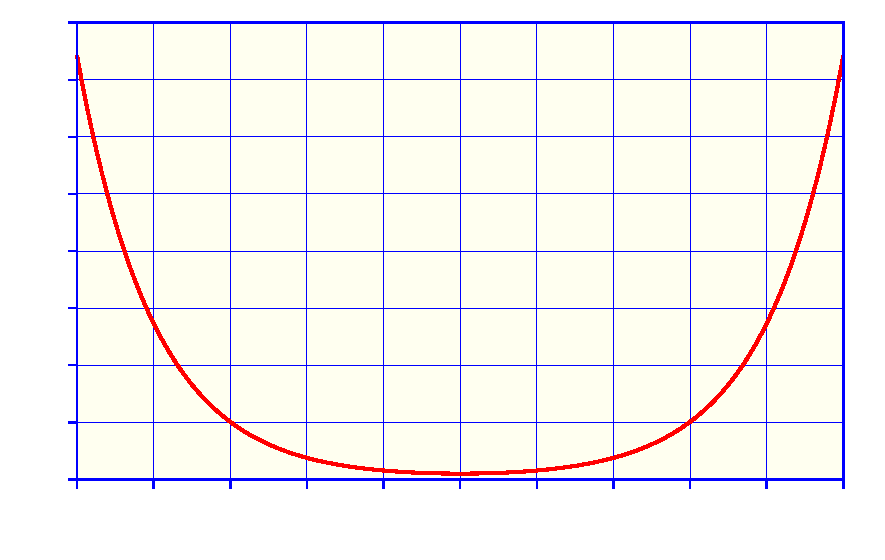
\includegraphics[width={425.00bp},height={269.00bp}]{Ape-Trigonometria-cosh}}%
    \gplfronttext
  \end{picture}%
\endgroup

	\captionof{figure}{Funció cosinus hiperbòlic} 
\end{center}

\vspace{5mm}
\begin{center}
	% GNUPLOT: LaTeX picture with Postscript
\begingroup
  \makeatletter
  \providecommand\color[2][]{%
    \GenericError{(gnuplot) \space\space\space\@spaces}{%
      Package color not loaded in conjunction with
      terminal option `colourtext'%
    }{See the gnuplot documentation for explanation.%
    }{Either use 'blacktext' in gnuplot or load the package
      color.sty in LaTeX.}%
    \renewcommand\color[2][]{}%
  }%
  \providecommand\includegraphics[2][]{%
    \GenericError{(gnuplot) \space\space\space\@spaces}{%
      Package graphicx or graphics not loaded%
    }{See the gnuplot documentation for explanation.%
    }{The gnuplot epslatex terminal needs graphicx.sty or graphics.sty.}%
    \renewcommand\includegraphics[2][]{}%
  }%
  \providecommand\rotatebox[2]{#2}%
  \@ifundefined{ifGPcolor}{%
    \newif\ifGPcolor
    \GPcolortrue
  }{}%
  \@ifundefined{ifGPblacktext}{%
    \newif\ifGPblacktext
    \GPblacktexttrue
  }{}%
  % define a \g@addto@macro without @ in the name:
  \let\gplgaddtomacro\g@addto@macro
  % define empty templates for all commands taking text:
  \gdef\gplbacktext{}%
  \gdef\gplfronttext{}%
  \makeatother
  \ifGPblacktext
    % no textcolor at all
    \def\colorrgb#1{}%
    \def\colorgray#1{}%
  \else
    % gray or color?
    \ifGPcolor
      \def\colorrgb#1{\color[rgb]{#1}}%
      \def\colorgray#1{\color[gray]{#1}}%
      \expandafter\def\csname LTw\endcsname{\color{white}}%
      \expandafter\def\csname LTb\endcsname{\color{black}}%
      \expandafter\def\csname LTa\endcsname{\color{black}}%
      \expandafter\def\csname LT0\endcsname{\color[rgb]{1,0,0}}%
      \expandafter\def\csname LT1\endcsname{\color[rgb]{0,1,0}}%
      \expandafter\def\csname LT2\endcsname{\color[rgb]{0,0,1}}%
      \expandafter\def\csname LT3\endcsname{\color[rgb]{1,0,1}}%
      \expandafter\def\csname LT4\endcsname{\color[rgb]{0,1,1}}%
      \expandafter\def\csname LT5\endcsname{\color[rgb]{1,1,0}}%
      \expandafter\def\csname LT6\endcsname{\color[rgb]{0,0,0}}%
      \expandafter\def\csname LT7\endcsname{\color[rgb]{1,0.3,0}}%
      \expandafter\def\csname LT8\endcsname{\color[rgb]{0.5,0.5,0.5}}%
    \else
      % gray
      \def\colorrgb#1{\color{black}}%
      \def\colorgray#1{\color[gray]{#1}}%
      \expandafter\def\csname LTw\endcsname{\color{white}}%
      \expandafter\def\csname LTb\endcsname{\color{black}}%
      \expandafter\def\csname LTa\endcsname{\color{black}}%
      \expandafter\def\csname LT0\endcsname{\color{black}}%
      \expandafter\def\csname LT1\endcsname{\color{black}}%
      \expandafter\def\csname LT2\endcsname{\color{black}}%
      \expandafter\def\csname LT3\endcsname{\color{black}}%
      \expandafter\def\csname LT4\endcsname{\color{black}}%
      \expandafter\def\csname LT5\endcsname{\color{black}}%
      \expandafter\def\csname LT6\endcsname{\color{black}}%
      \expandafter\def\csname LT7\endcsname{\color{black}}%
      \expandafter\def\csname LT8\endcsname{\color{black}}%
    \fi
  \fi
    \setlength{\unitlength}{0.0500bp}%
    \ifx\gptboxheight\undefined%
      \newlength{\gptboxheight}%
      \newlength{\gptboxwidth}%
      \newsavebox{\gptboxtext}%
    \fi%
    \setlength{\fboxrule}{0.5pt}%
    \setlength{\fboxsep}{1pt}%
    \definecolor{tbcol}{rgb}{1,1,1}%
\begin{picture}(8500.00,5380.00)%
    \gplgaddtomacro\gplbacktext{%
      \colorrgb{0.00,0.00,0.00}%%
      \put(740,764){\makebox(0,0)[r]{\strut{} 0,0}}%
      \colorrgb{0.00,0.00,0.00}%%
      \put(740,1202){\makebox(0,0)[r]{\strut{} 0,1}}%
      \colorrgb{0.00,0.00,0.00}%%
      \put(740,1641){\makebox(0,0)[r]{\strut{} 0,2}}%
      \colorrgb{0.00,0.00,0.00}%%
      \put(740,2079){\makebox(0,0)[r]{\strut{} 0,3}}%
      \colorrgb{0.00,0.00,0.00}%%
      \put(740,2517){\makebox(0,0)[r]{\strut{} 0,4}}%
      \colorrgb{0.00,0.00,0.00}%%
      \put(740,2956){\makebox(0,0)[r]{\strut{} 0,5}}%
      \colorrgb{0.00,0.00,0.00}%%
      \put(740,3394){\makebox(0,0)[r]{\strut{} 0,6}}%
      \colorrgb{0.00,0.00,0.00}%%
      \put(740,3832){\makebox(0,0)[r]{\strut{} 0,7}}%
      \colorrgb{0.00,0.00,0.00}%%
      \put(740,4270){\makebox(0,0)[r]{\strut{} 0,8}}%
      \colorrgb{0.00,0.00,0.00}%%
      \put(740,4709){\makebox(0,0)[r]{\strut{} 0,9}}%
      \colorrgb{0.00,0.00,0.00}%%
      \put(740,5147){\makebox(0,0)[r]{\strut{} 1,0}}%
      \colorrgb{0.00,0.00,0.00}%%
      \put(921,467){\makebox(0,0){\strut{}-5}}%
      \colorrgb{0.00,0.00,0.00}%%
      \put(1638,467){\makebox(0,0){\strut{}-4}}%
      \colorrgb{0.00,0.00,0.00}%%
      \put(2354,467){\makebox(0,0){\strut{}-3}}%
      \colorrgb{0.00,0.00,0.00}%%
      \put(3071,467){\makebox(0,0){\strut{}-2}}%
      \colorrgb{0.00,0.00,0.00}%%
      \put(3787,467){\makebox(0,0){\strut{}-1}}%
      \colorrgb{0.00,0.00,0.00}%%
      \put(4503,467){\makebox(0,0){\strut{} 0}}%
      \colorrgb{0.00,0.00,0.00}%%
      \put(5220,467){\makebox(0,0){\strut{} 1}}%
      \colorrgb{0.00,0.00,0.00}%%
      \put(5936,467){\makebox(0,0){\strut{} 2}}%
      \colorrgb{0.00,0.00,0.00}%%
      \put(6652,467){\makebox(0,0){\strut{} 3}}%
      \colorrgb{0.00,0.00,0.00}%%
      \put(7369,467){\makebox(0,0){\strut{} 4}}%
      \colorrgb{0.00,0.00,0.00}%%
      \put(8085,467){\makebox(0,0){\strut{} 5}}%
    }%
    \gplgaddtomacro\gplfronttext{%
      \csname LTb\endcsname%%
      \put(178,2956){\rotatebox{-270}{\makebox(0,0){\strut{}$\sech z$}}}%
      \csname LTb\endcsname%%
      \put(8138,2956){\rotatebox{-270}{\makebox(0,0){\strut{}}}}%
      \csname LTb\endcsname%%
      \put(4503,148){\makebox(0,0){\strut{}$z$}}%
      \csname LTb\endcsname%%
      \put(4503,5147){\makebox(0,0){\strut{}}}%
      \csname LTb\endcsname%%
      \put(4503,5147){\makebox(0,0){\strut{}}}%
    }%
    \gplbacktext
    \put(0,0){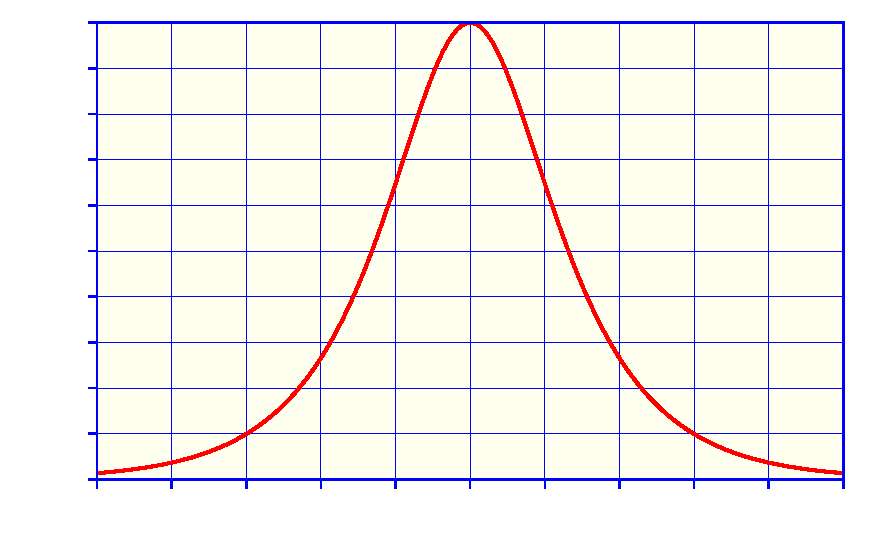
\includegraphics[width={425.00bp},height={269.00bp}]{Ape-Trigonometria-sech}}%
    \gplfronttext
  \end{picture}%
\endgroup

	\captionof{figure}{Funció secant hiperbòlica} 
\end{center}

\begin{center}
	% GNUPLOT: LaTeX picture with Postscript
\begingroup
  \makeatletter
  \providecommand\color[2][]{%
    \GenericError{(gnuplot) \space\space\space\@spaces}{%
      Package color not loaded in conjunction with
      terminal option `colourtext'%
    }{See the gnuplot documentation for explanation.%
    }{Either use 'blacktext' in gnuplot or load the package
      color.sty in LaTeX.}%
    \renewcommand\color[2][]{}%
  }%
  \providecommand\includegraphics[2][]{%
    \GenericError{(gnuplot) \space\space\space\@spaces}{%
      Package graphicx or graphics not loaded%
    }{See the gnuplot documentation for explanation.%
    }{The gnuplot epslatex terminal needs graphicx.sty or graphics.sty.}%
    \renewcommand\includegraphics[2][]{}%
  }%
  \providecommand\rotatebox[2]{#2}%
  \@ifundefined{ifGPcolor}{%
    \newif\ifGPcolor
    \GPcolortrue
  }{}%
  \@ifundefined{ifGPblacktext}{%
    \newif\ifGPblacktext
    \GPblacktexttrue
  }{}%
  % define a \g@addto@macro without @ in the name:
  \let\gplgaddtomacro\g@addto@macro
  % define empty templates for all commands taking text:
  \gdef\gplbacktext{}%
  \gdef\gplfronttext{}%
  \makeatother
  \ifGPblacktext
    % no textcolor at all
    \def\colorrgb#1{}%
    \def\colorgray#1{}%
  \else
    % gray or color?
    \ifGPcolor
      \def\colorrgb#1{\color[rgb]{#1}}%
      \def\colorgray#1{\color[gray]{#1}}%
      \expandafter\def\csname LTw\endcsname{\color{white}}%
      \expandafter\def\csname LTb\endcsname{\color{black}}%
      \expandafter\def\csname LTa\endcsname{\color{black}}%
      \expandafter\def\csname LT0\endcsname{\color[rgb]{1,0,0}}%
      \expandafter\def\csname LT1\endcsname{\color[rgb]{0,1,0}}%
      \expandafter\def\csname LT2\endcsname{\color[rgb]{0,0,1}}%
      \expandafter\def\csname LT3\endcsname{\color[rgb]{1,0,1}}%
      \expandafter\def\csname LT4\endcsname{\color[rgb]{0,1,1}}%
      \expandafter\def\csname LT5\endcsname{\color[rgb]{1,1,0}}%
      \expandafter\def\csname LT6\endcsname{\color[rgb]{0,0,0}}%
      \expandafter\def\csname LT7\endcsname{\color[rgb]{1,0.3,0}}%
      \expandafter\def\csname LT8\endcsname{\color[rgb]{0.5,0.5,0.5}}%
    \else
      % gray
      \def\colorrgb#1{\color{black}}%
      \def\colorgray#1{\color[gray]{#1}}%
      \expandafter\def\csname LTw\endcsname{\color{white}}%
      \expandafter\def\csname LTb\endcsname{\color{black}}%
      \expandafter\def\csname LTa\endcsname{\color{black}}%
      \expandafter\def\csname LT0\endcsname{\color{black}}%
      \expandafter\def\csname LT1\endcsname{\color{black}}%
      \expandafter\def\csname LT2\endcsname{\color{black}}%
      \expandafter\def\csname LT3\endcsname{\color{black}}%
      \expandafter\def\csname LT4\endcsname{\color{black}}%
      \expandafter\def\csname LT5\endcsname{\color{black}}%
      \expandafter\def\csname LT6\endcsname{\color{black}}%
      \expandafter\def\csname LT7\endcsname{\color{black}}%
      \expandafter\def\csname LT8\endcsname{\color{black}}%
    \fi
  \fi
    \setlength{\unitlength}{0.0500bp}%
    \ifx\gptboxheight\undefined%
      \newlength{\gptboxheight}%
      \newlength{\gptboxwidth}%
      \newsavebox{\gptboxtext}%
    \fi%
    \setlength{\fboxrule}{0.5pt}%
    \setlength{\fboxsep}{1pt}%
    \definecolor{tbcol}{rgb}{1,1,1}%
\begin{picture}(8500.00,5380.00)%
    \gplgaddtomacro\gplbacktext{%
      \colorrgb{0.00,0.00,0.00}%%
      \put(837,764){\makebox(0,0)[r]{\strut{}-1,00}}%
      \colorrgb{0.00,0.00,0.00}%%
      \put(837,1312){\makebox(0,0)[r]{\strut{}-0,75}}%
      \colorrgb{0.00,0.00,0.00}%%
      \put(837,1860){\makebox(0,0)[r]{\strut{}-0,50}}%
      \colorrgb{0.00,0.00,0.00}%%
      \put(837,2408){\makebox(0,0)[r]{\strut{}-0,25}}%
      \colorrgb{0.00,0.00,0.00}%%
      \put(837,2956){\makebox(0,0)[r]{\strut{} 0,00}}%
      \colorrgb{0.00,0.00,0.00}%%
      \put(837,3503){\makebox(0,0)[r]{\strut{} 0,25}}%
      \colorrgb{0.00,0.00,0.00}%%
      \put(837,4051){\makebox(0,0)[r]{\strut{} 0,50}}%
      \colorrgb{0.00,0.00,0.00}%%
      \put(837,4599){\makebox(0,0)[r]{\strut{} 0,75}}%
      \colorrgb{0.00,0.00,0.00}%%
      \put(837,5147){\makebox(0,0)[r]{\strut{} 1,00}}%
      \colorrgb{0.00,0.00,0.00}%%
      \put(1018,467){\makebox(0,0){\strut{}-5}}%
      \colorrgb{0.00,0.00,0.00}%%
      \put(1724,467){\makebox(0,0){\strut{}-4}}%
      \colorrgb{0.00,0.00,0.00}%%
      \put(2431,467){\makebox(0,0){\strut{}-3}}%
      \colorrgb{0.00,0.00,0.00}%%
      \put(3138,467){\makebox(0,0){\strut{}-2}}%
      \colorrgb{0.00,0.00,0.00}%%
      \put(3845,467){\makebox(0,0){\strut{}-1}}%
      \colorrgb{0.00,0.00,0.00}%%
      \put(4551,467){\makebox(0,0){\strut{} 0}}%
      \colorrgb{0.00,0.00,0.00}%%
      \put(5258,467){\makebox(0,0){\strut{} 1}}%
      \colorrgb{0.00,0.00,0.00}%%
      \put(5965,467){\makebox(0,0){\strut{} 2}}%
      \colorrgb{0.00,0.00,0.00}%%
      \put(6671,467){\makebox(0,0){\strut{} 3}}%
      \colorrgb{0.00,0.00,0.00}%%
      \put(7378,467){\makebox(0,0){\strut{} 4}}%
      \colorrgb{0.00,0.00,0.00}%%
      \put(8085,467){\makebox(0,0){\strut{} 5}}%
    }%
    \gplgaddtomacro\gplfronttext{%
      \csname LTb\endcsname%%
      \put(178,2956){\rotatebox{-270}{\makebox(0,0){\strut{}$\tanh z$}}}%
      \csname LTb\endcsname%%
      \put(8138,2956){\rotatebox{-270}{\makebox(0,0){\strut{}}}}%
      \csname LTb\endcsname%%
      \put(4551,148){\makebox(0,0){\strut{}$z$}}%
      \csname LTb\endcsname%%
      \put(4551,5147){\makebox(0,0){\strut{}}}%
      \csname LTb\endcsname%%
      \put(4551,5147){\makebox(0,0){\strut{}}}%
    }%
    \gplbacktext
    \put(0,0){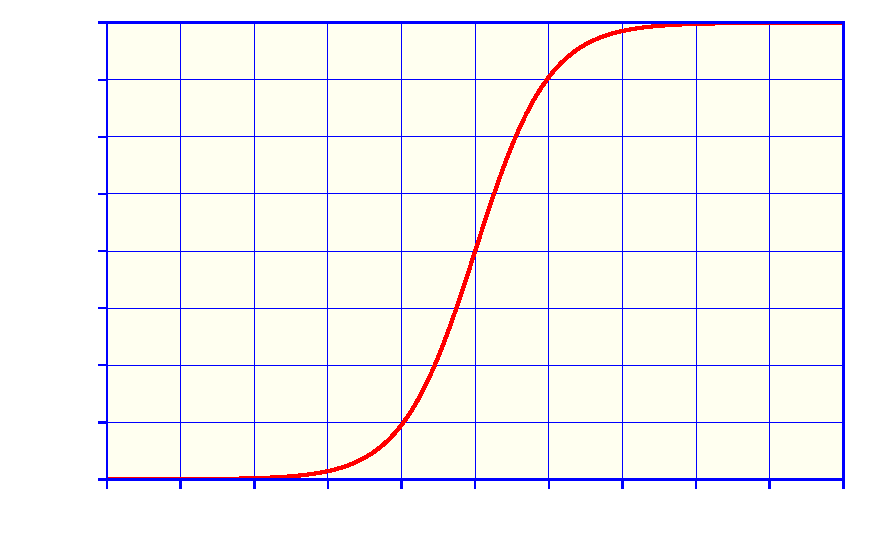
\includegraphics[width={425.00bp},height={269.00bp}]{Ape-Trigonometria-tanh}}%
    \gplfronttext
  \end{picture}%
\endgroup

	\captionof{figure}{Funció tangent hiperbòlica} 
\end{center}

\vspace{5mm}
\begin{center}
	% GNUPLOT: LaTeX picture with Postscript
\begingroup
  \makeatletter
  \providecommand\color[2][]{%
    \GenericError{(gnuplot) \space\space\space\@spaces}{%
      Package color not loaded in conjunction with
      terminal option `colourtext'%
    }{See the gnuplot documentation for explanation.%
    }{Either use 'blacktext' in gnuplot or load the package
      color.sty in LaTeX.}%
    \renewcommand\color[2][]{}%
  }%
  \providecommand\includegraphics[2][]{%
    \GenericError{(gnuplot) \space\space\space\@spaces}{%
      Package graphicx or graphics not loaded%
    }{See the gnuplot documentation for explanation.%
    }{The gnuplot epslatex terminal needs graphicx.sty or graphics.sty.}%
    \renewcommand\includegraphics[2][]{}%
  }%
  \providecommand\rotatebox[2]{#2}%
  \@ifundefined{ifGPcolor}{%
    \newif\ifGPcolor
    \GPcolortrue
  }{}%
  \@ifundefined{ifGPblacktext}{%
    \newif\ifGPblacktext
    \GPblacktexttrue
  }{}%
  % define a \g@addto@macro without @ in the name:
  \let\gplgaddtomacro\g@addto@macro
  % define empty templates for all commands taking text:
  \gdef\gplbacktext{}%
  \gdef\gplfronttext{}%
  \makeatother
  \ifGPblacktext
    % no textcolor at all
    \def\colorrgb#1{}%
    \def\colorgray#1{}%
  \else
    % gray or color?
    \ifGPcolor
      \def\colorrgb#1{\color[rgb]{#1}}%
      \def\colorgray#1{\color[gray]{#1}}%
      \expandafter\def\csname LTw\endcsname{\color{white}}%
      \expandafter\def\csname LTb\endcsname{\color{black}}%
      \expandafter\def\csname LTa\endcsname{\color{black}}%
      \expandafter\def\csname LT0\endcsname{\color[rgb]{1,0,0}}%
      \expandafter\def\csname LT1\endcsname{\color[rgb]{0,1,0}}%
      \expandafter\def\csname LT2\endcsname{\color[rgb]{0,0,1}}%
      \expandafter\def\csname LT3\endcsname{\color[rgb]{1,0,1}}%
      \expandafter\def\csname LT4\endcsname{\color[rgb]{0,1,1}}%
      \expandafter\def\csname LT5\endcsname{\color[rgb]{1,1,0}}%
      \expandafter\def\csname LT6\endcsname{\color[rgb]{0,0,0}}%
      \expandafter\def\csname LT7\endcsname{\color[rgb]{1,0.3,0}}%
      \expandafter\def\csname LT8\endcsname{\color[rgb]{0.5,0.5,0.5}}%
    \else
      % gray
      \def\colorrgb#1{\color{black}}%
      \def\colorgray#1{\color[gray]{#1}}%
      \expandafter\def\csname LTw\endcsname{\color{white}}%
      \expandafter\def\csname LTb\endcsname{\color{black}}%
      \expandafter\def\csname LTa\endcsname{\color{black}}%
      \expandafter\def\csname LT0\endcsname{\color{black}}%
      \expandafter\def\csname LT1\endcsname{\color{black}}%
      \expandafter\def\csname LT2\endcsname{\color{black}}%
      \expandafter\def\csname LT3\endcsname{\color{black}}%
      \expandafter\def\csname LT4\endcsname{\color{black}}%
      \expandafter\def\csname LT5\endcsname{\color{black}}%
      \expandafter\def\csname LT6\endcsname{\color{black}}%
      \expandafter\def\csname LT7\endcsname{\color{black}}%
      \expandafter\def\csname LT8\endcsname{\color{black}}%
    \fi
  \fi
    \setlength{\unitlength}{0.0500bp}%
    \ifx\gptboxheight\undefined%
      \newlength{\gptboxheight}%
      \newlength{\gptboxwidth}%
      \newsavebox{\gptboxtext}%
    \fi%
    \setlength{\fboxrule}{0.5pt}%
    \setlength{\fboxsep}{1pt}%
    \definecolor{tbcol}{rgb}{1,1,1}%
\begin{picture}(8500.00,5380.00)%
    \gplgaddtomacro\gplbacktext{%
      \colorrgb{0.00,0.00,0.00}%%
      \put(548,764){\makebox(0,0)[r]{\strut{}-5}}%
      \colorrgb{0.00,0.00,0.00}%%
      \put(548,1202){\makebox(0,0)[r]{\strut{}-4}}%
      \colorrgb{0.00,0.00,0.00}%%
      \put(548,1641){\makebox(0,0)[r]{\strut{}-3}}%
      \colorrgb{0.00,0.00,0.00}%%
      \put(548,2079){\makebox(0,0)[r]{\strut{}-2}}%
      \colorrgb{0.00,0.00,0.00}%%
      \put(548,2517){\makebox(0,0)[r]{\strut{}-1}}%
      \colorrgb{0.00,0.00,0.00}%%
      \put(548,2956){\makebox(0,0)[r]{\strut{} 0}}%
      \colorrgb{0.00,0.00,0.00}%%
      \put(548,3394){\makebox(0,0)[r]{\strut{} 1}}%
      \colorrgb{0.00,0.00,0.00}%%
      \put(548,3832){\makebox(0,0)[r]{\strut{} 2}}%
      \colorrgb{0.00,0.00,0.00}%%
      \put(548,4270){\makebox(0,0)[r]{\strut{} 3}}%
      \colorrgb{0.00,0.00,0.00}%%
      \put(548,4709){\makebox(0,0)[r]{\strut{} 4}}%
      \colorrgb{0.00,0.00,0.00}%%
      \put(548,5147){\makebox(0,0)[r]{\strut{} 5}}%
      \colorrgb{0.00,0.00,0.00}%%
      \put(729,467){\makebox(0,0){\strut{}-5}}%
      \colorrgb{0.00,0.00,0.00}%%
      \put(1465,467){\makebox(0,0){\strut{}-4}}%
      \colorrgb{0.00,0.00,0.00}%%
      \put(2200,467){\makebox(0,0){\strut{}-3}}%
      \colorrgb{0.00,0.00,0.00}%%
      \put(2936,467){\makebox(0,0){\strut{}-2}}%
      \colorrgb{0.00,0.00,0.00}%%
      \put(3672,467){\makebox(0,0){\strut{}-1}}%
      \colorrgb{0.00,0.00,0.00}%%
      \put(4407,467){\makebox(0,0){\strut{} 0}}%
      \colorrgb{0.00,0.00,0.00}%%
      \put(5143,467){\makebox(0,0){\strut{} 1}}%
      \colorrgb{0.00,0.00,0.00}%%
      \put(5878,467){\makebox(0,0){\strut{} 2}}%
      \colorrgb{0.00,0.00,0.00}%%
      \put(6614,467){\makebox(0,0){\strut{} 3}}%
      \colorrgb{0.00,0.00,0.00}%%
      \put(7349,467){\makebox(0,0){\strut{} 4}}%
      \colorrgb{0.00,0.00,0.00}%%
      \put(8085,467){\makebox(0,0){\strut{} 5}}%
    }%
    \gplgaddtomacro\gplfronttext{%
      \csname LTb\endcsname%%
      \put(178,2956){\rotatebox{-270}{\makebox(0,0){\strut{}$\coth z$}}}%
      \csname LTb\endcsname%%
      \put(8138,2956){\rotatebox{-270}{\makebox(0,0){\strut{}}}}%
      \csname LTb\endcsname%%
      \put(4407,148){\makebox(0,0){\strut{}$z$}}%
      \csname LTb\endcsname%%
      \put(4407,5147){\makebox(0,0){\strut{}}}%
      \csname LTb\endcsname%%
      \put(4407,5147){\makebox(0,0){\strut{}}}%
    }%
    \gplbacktext
    \put(0,0){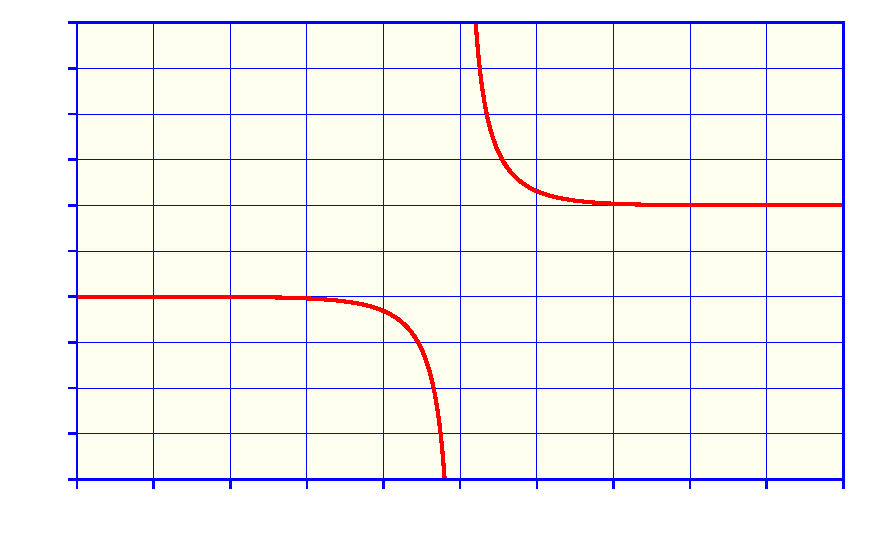
\includegraphics[width={425.00bp},height={269.00bp}]{Ape-Trigonometria-coth}}%
    \gplfronttext
  \end{picture}%
\endgroup

	\captionof{figure}{Funció cotangent hiperbòlica} 
\end{center}